% Appendix1 file from standard thesis template

\appendixtitle 
\appendix

%% Use the following two lines for single appendix
\unappendixtitle
\singleappendixtitle

\chapter{}

\begin{figure}\
  \begin{subfigure}[b]{0.49\textwidth}
    \centering
    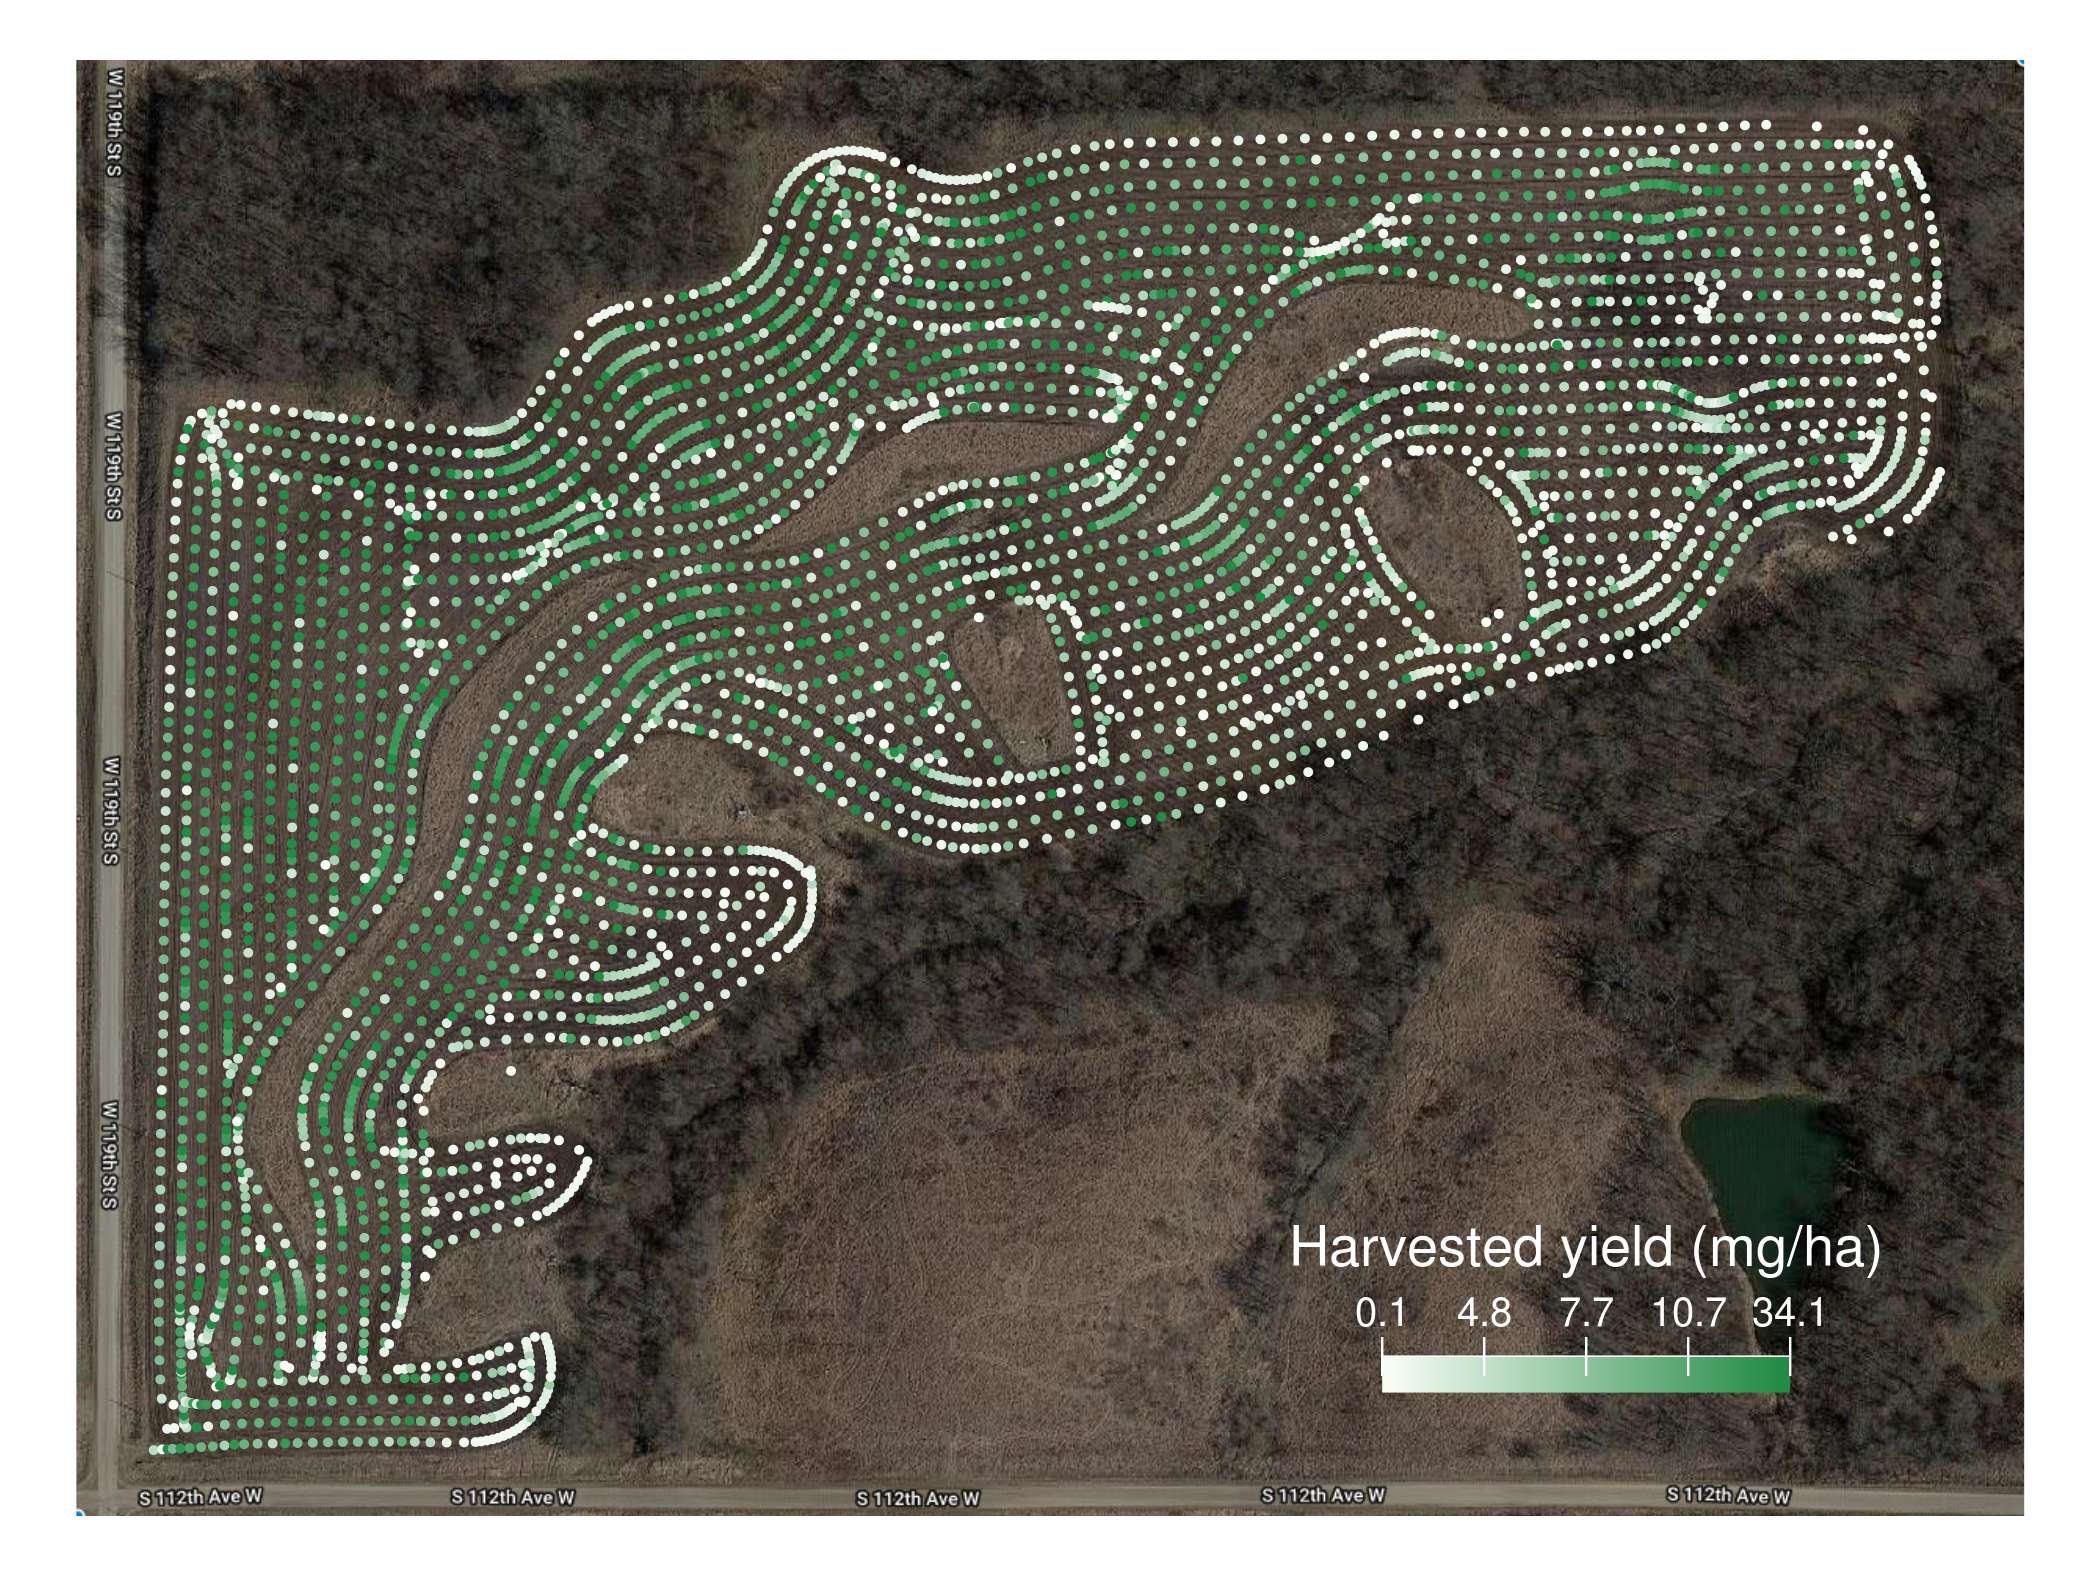
\includegraphics[width=1\textwidth]{appendix/basswood_2012_res5_1_points_vehicle}
   \end{subfigure}
  \begin{subfigure}[b]{0.49\textwidth}
    \centering
    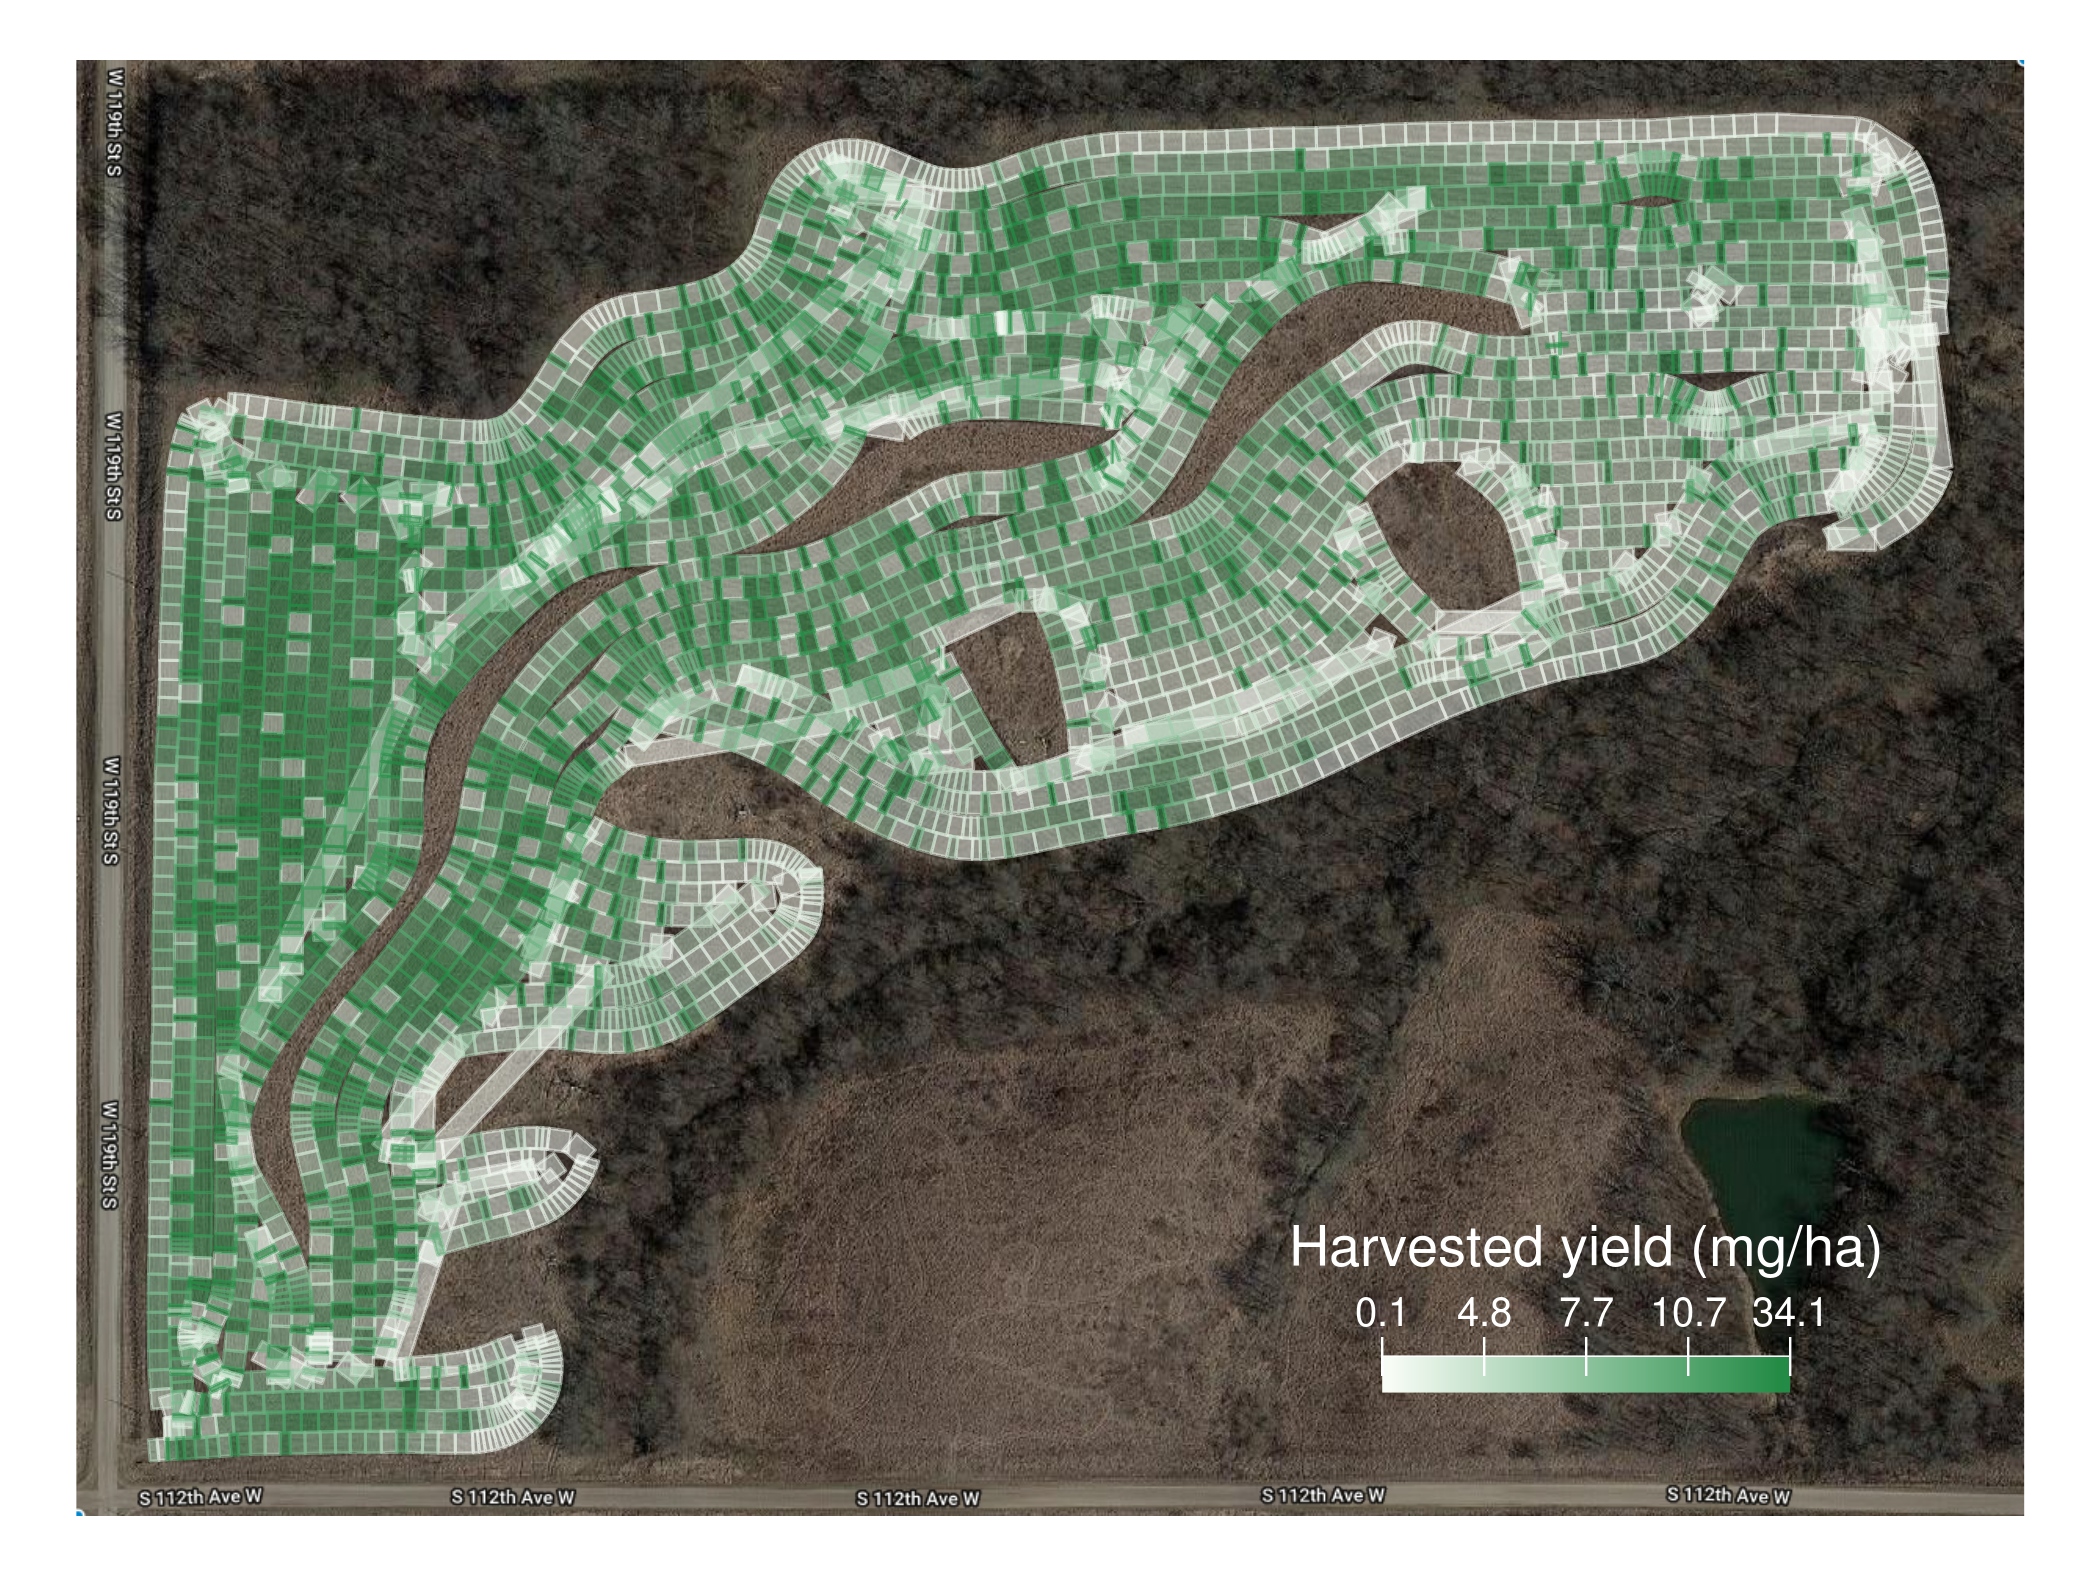
\includegraphics[width=1\textwidth]{appendix/basswood_2012_res5_1_polygons_vehicle}
  \end{subfigure}
  \begin{subfigure}[b]{0.49\textwidth}
    \centering
    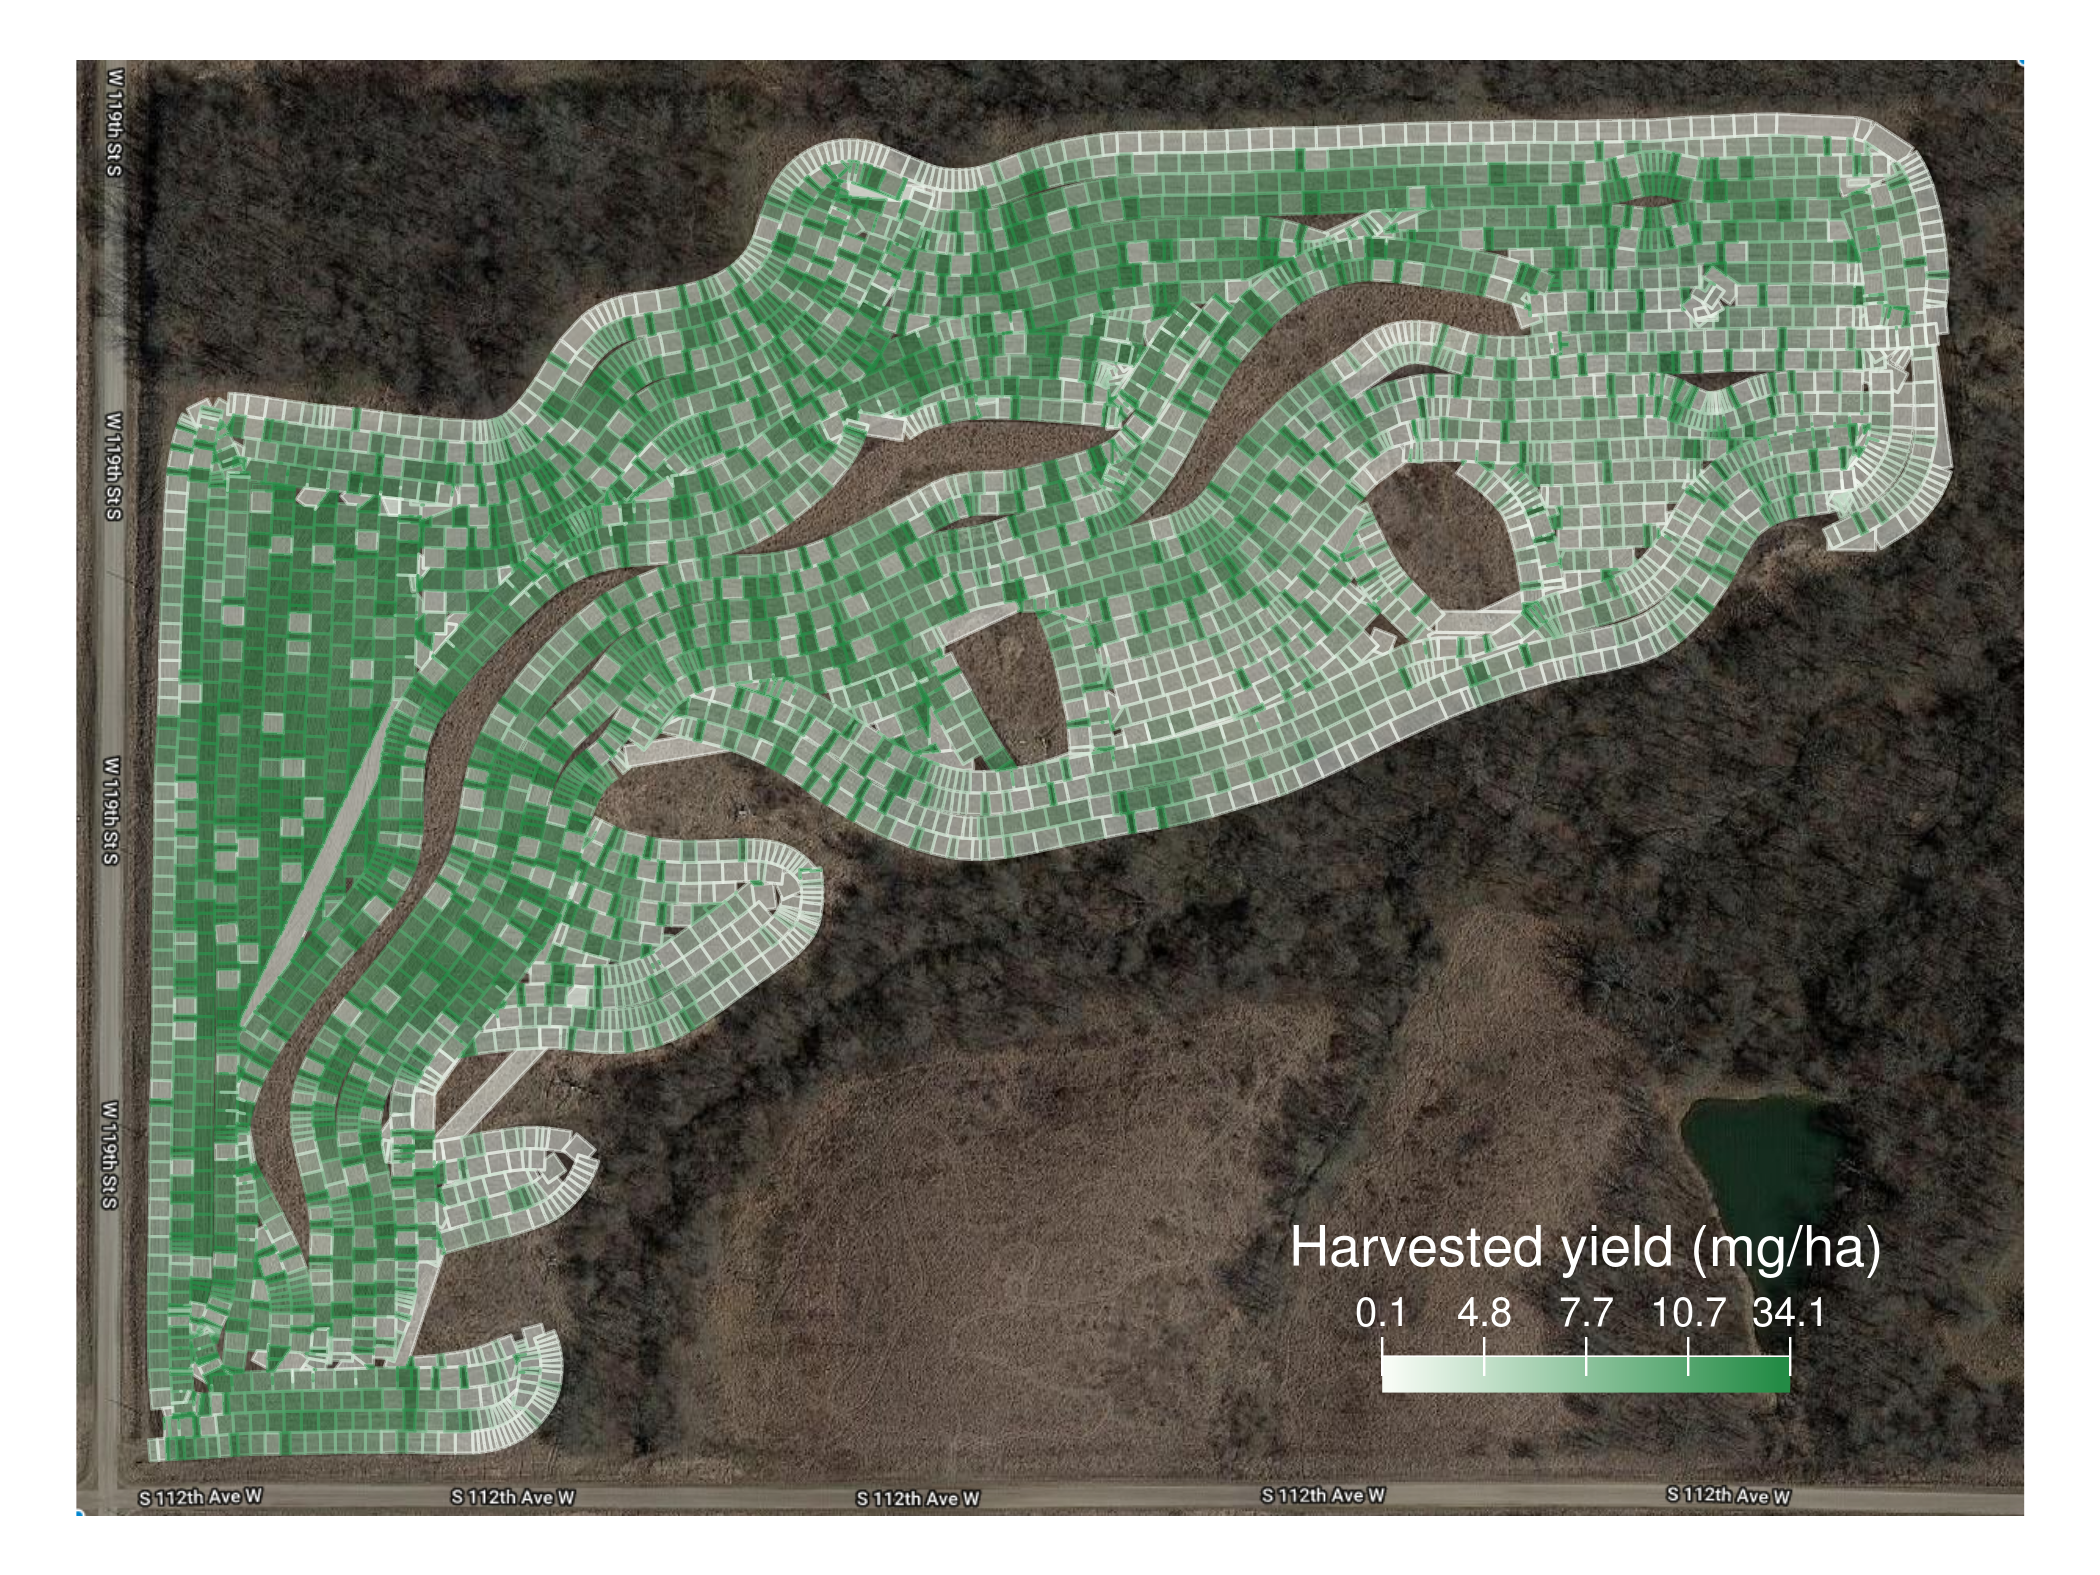
\includegraphics[width=1\textwidth]{appendix/basswood_2012_res5_1_reshaped}
  \end{subfigure}
  \begin{subfigure}[b]{0.49\textwidth}
    \centering
    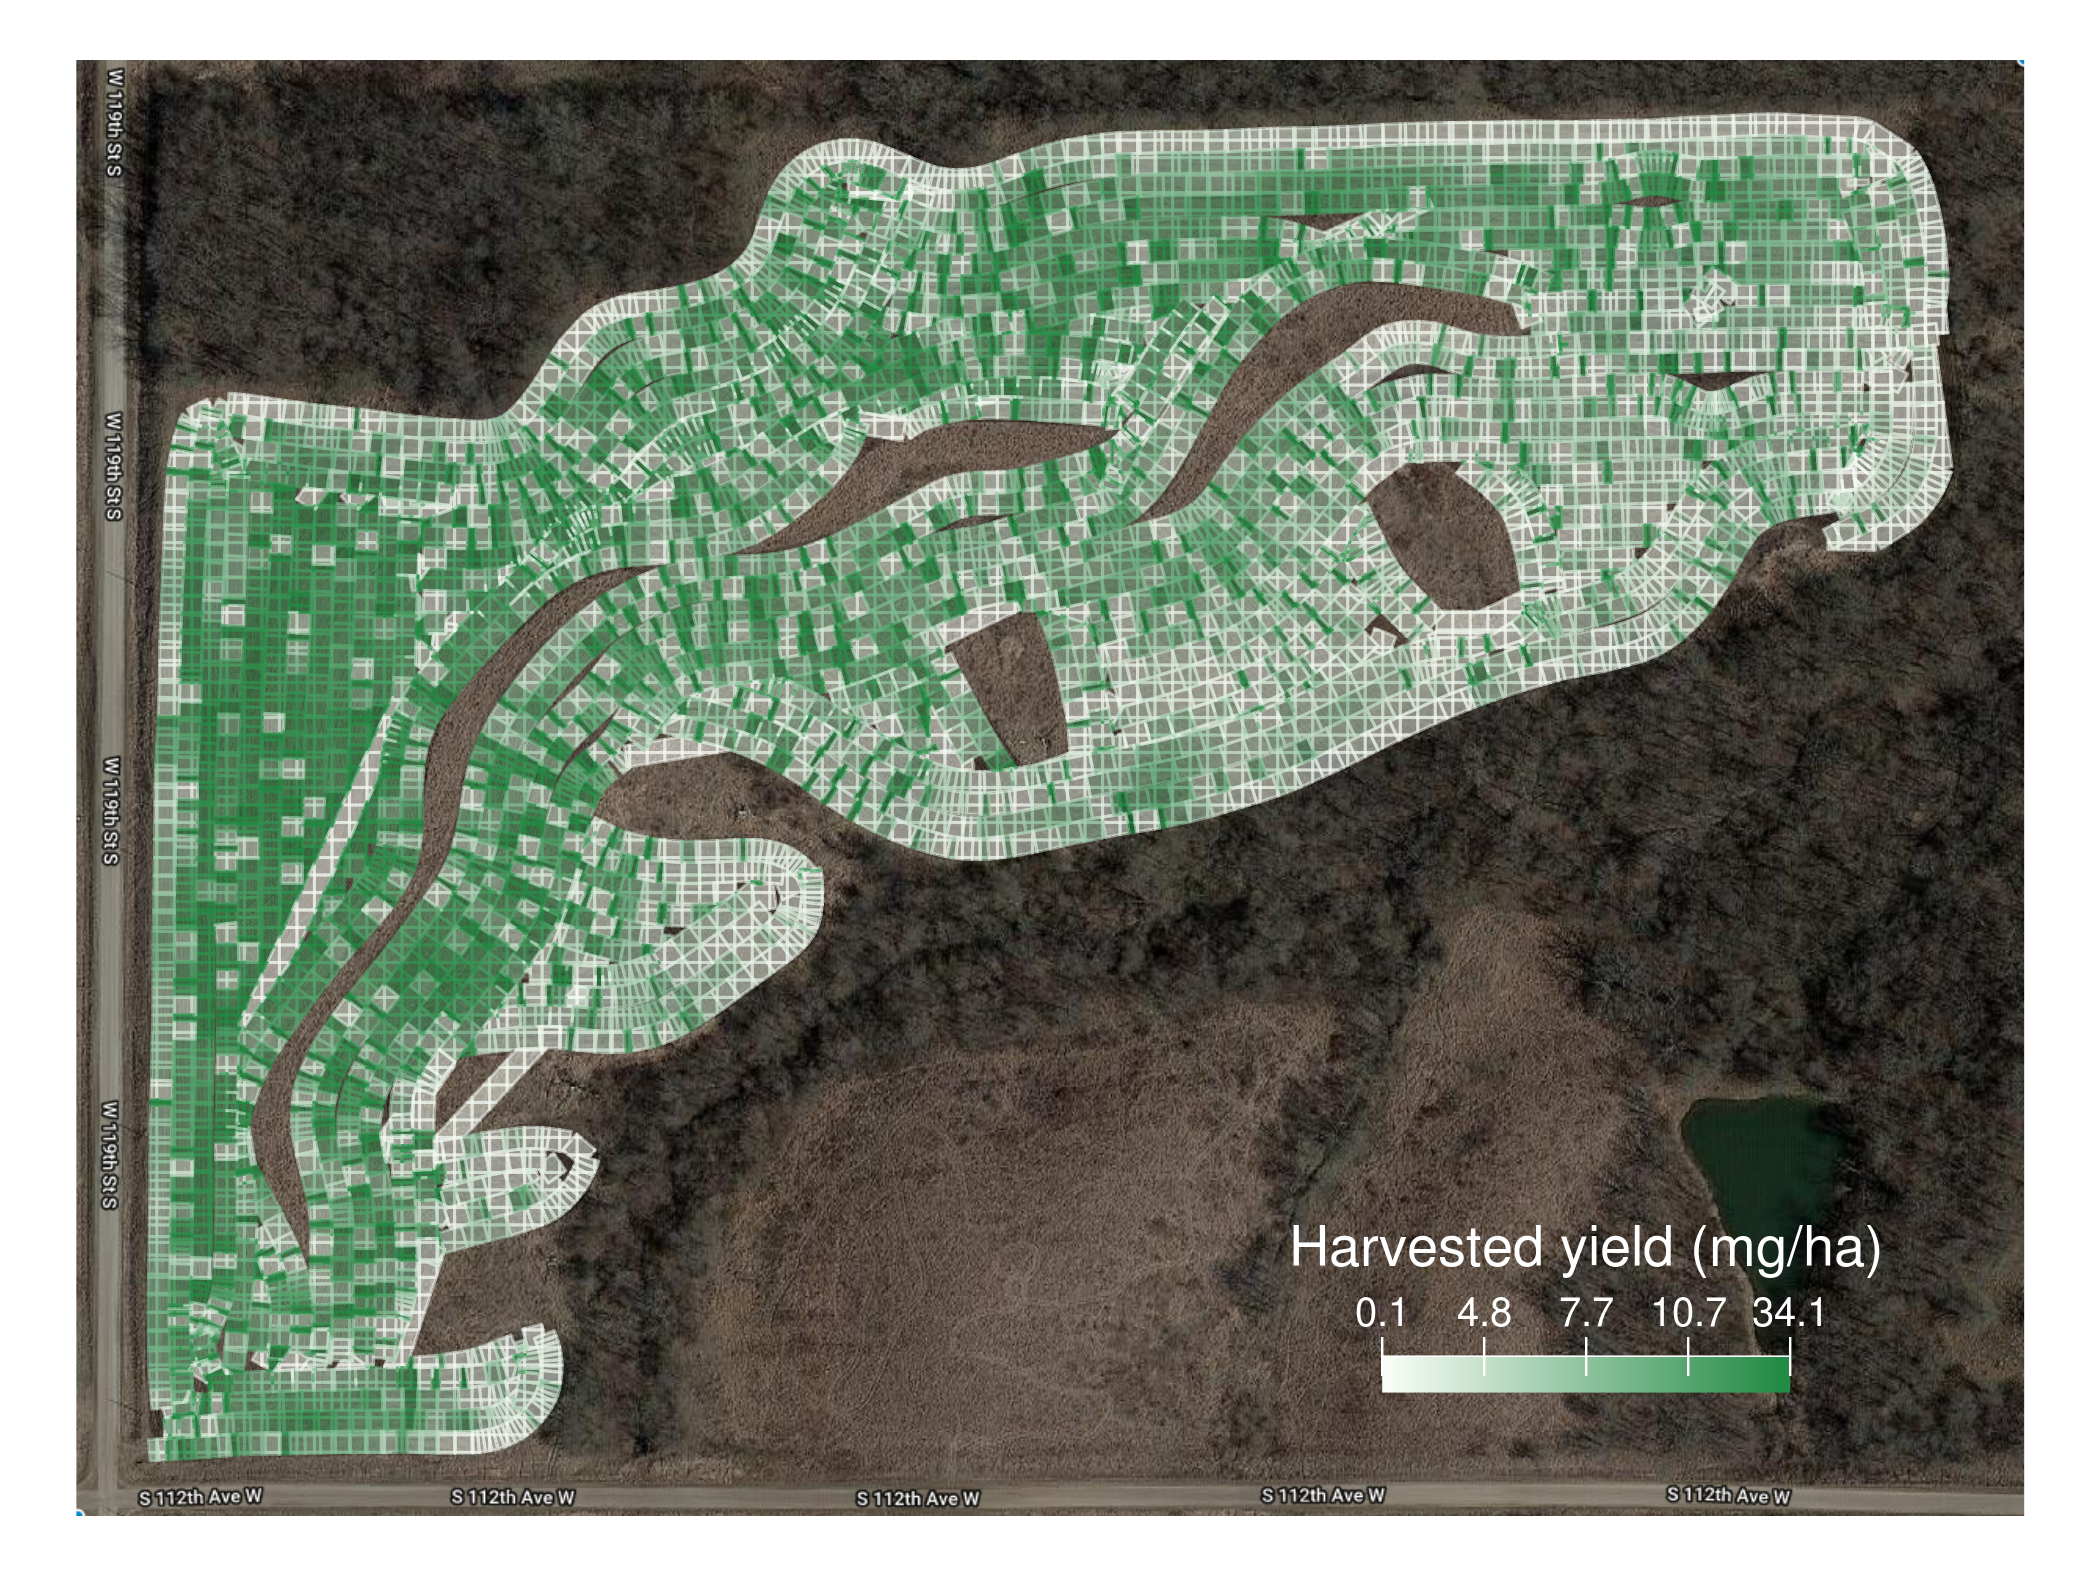
\includegraphics[width=1\textwidth]{appendix/basswood_2012_res5_1_chopped}
   \end{subfigure}
  \begin{subfigure}[b]{0.49\textwidth}
    \centering
    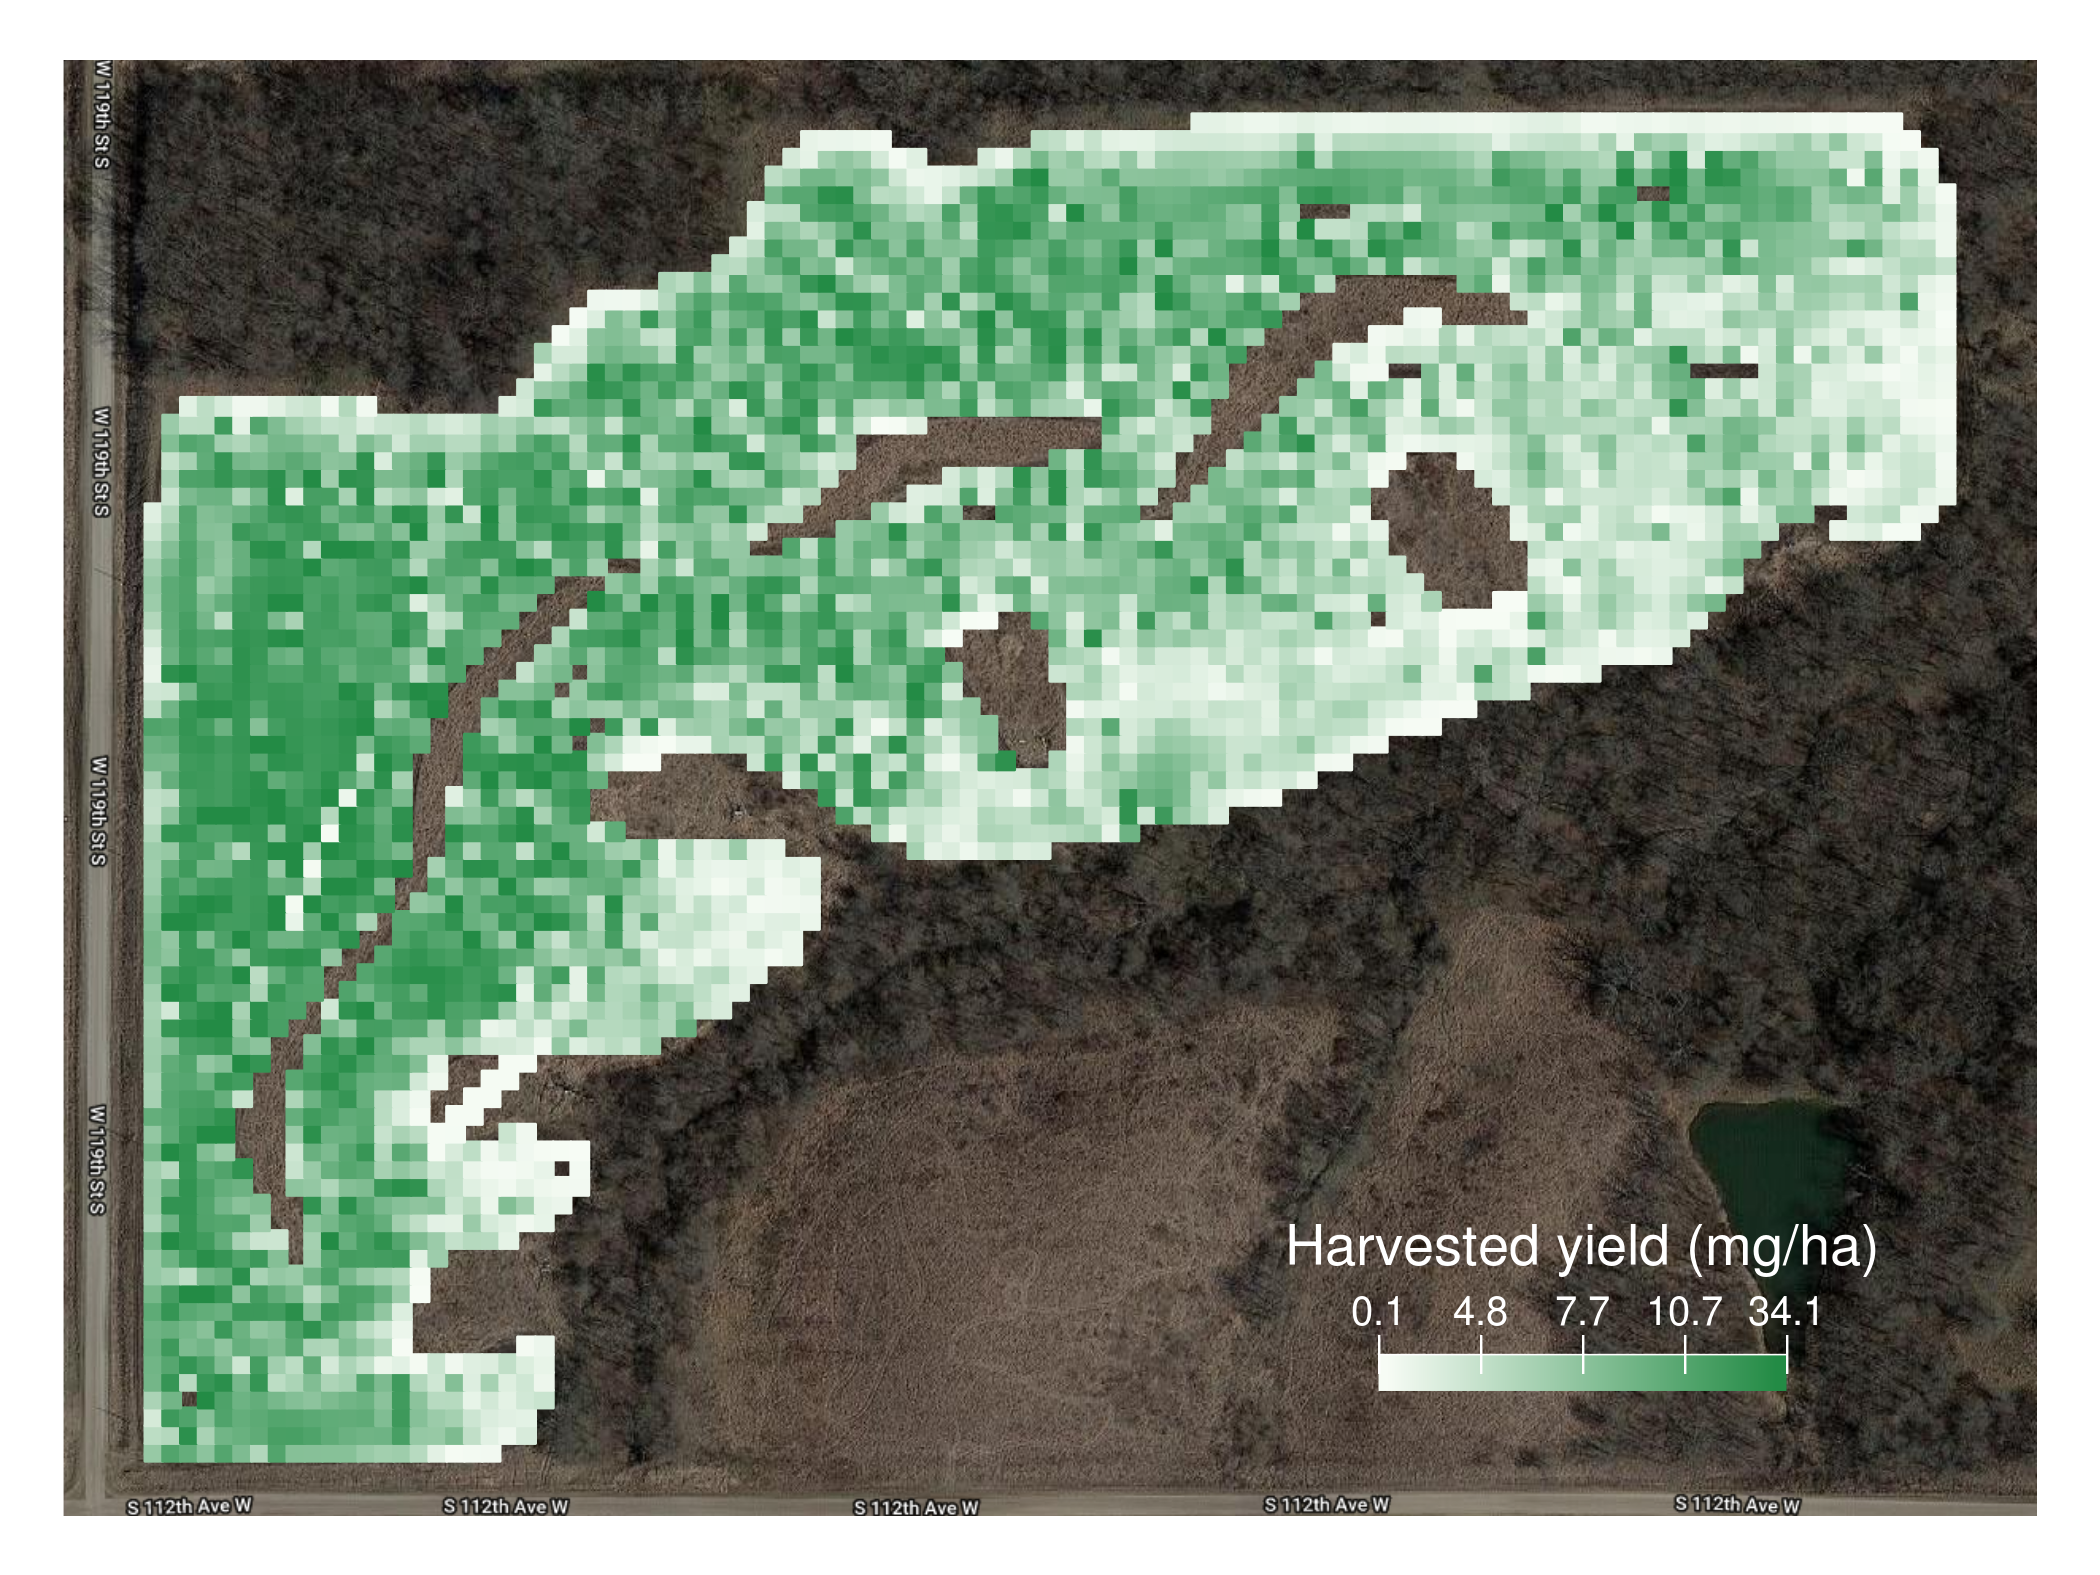
\includegraphics[width=1\textwidth]{appendix/basswood_2012_res5_1_aggregated}
   \end{subfigure}
  \begin{subfigure}[b]{0.49\textwidth}
    \centering
    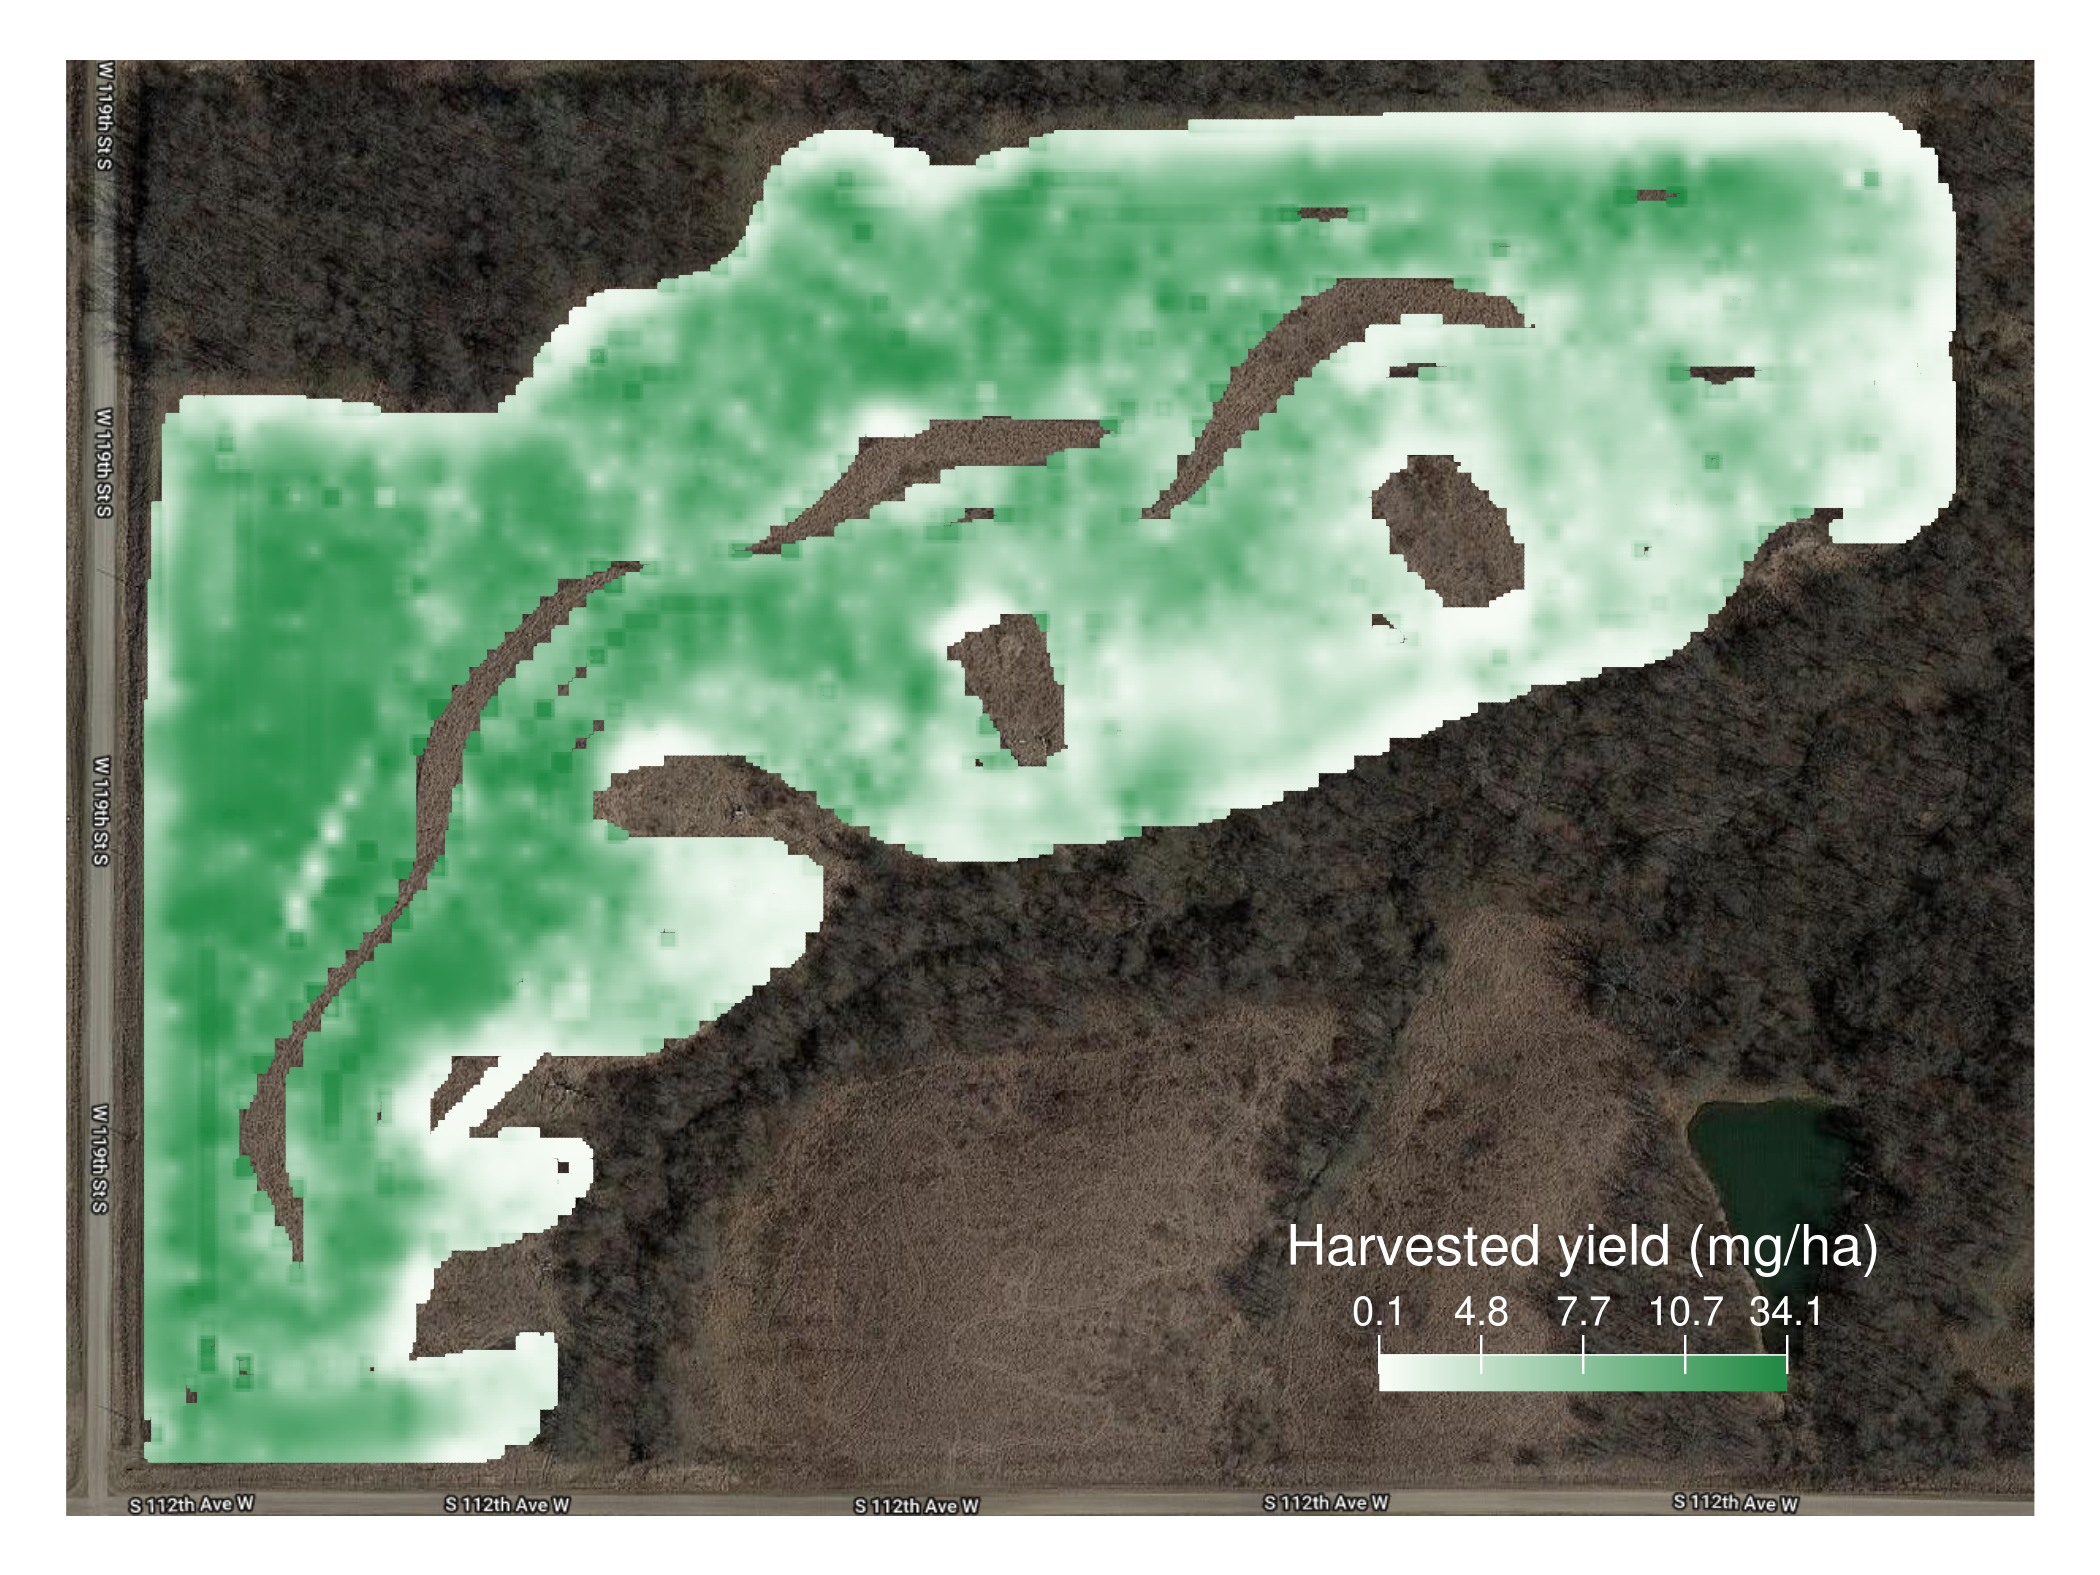
\includegraphics[width=1\textwidth]{appendix/basswood_2012_res5_1_smoothed}
  \end{subfigure}
\end{figure}

% \begin{figure}
%     \centering
%     \begin{minipage}{0.49\textwidth}
%         \centering
%         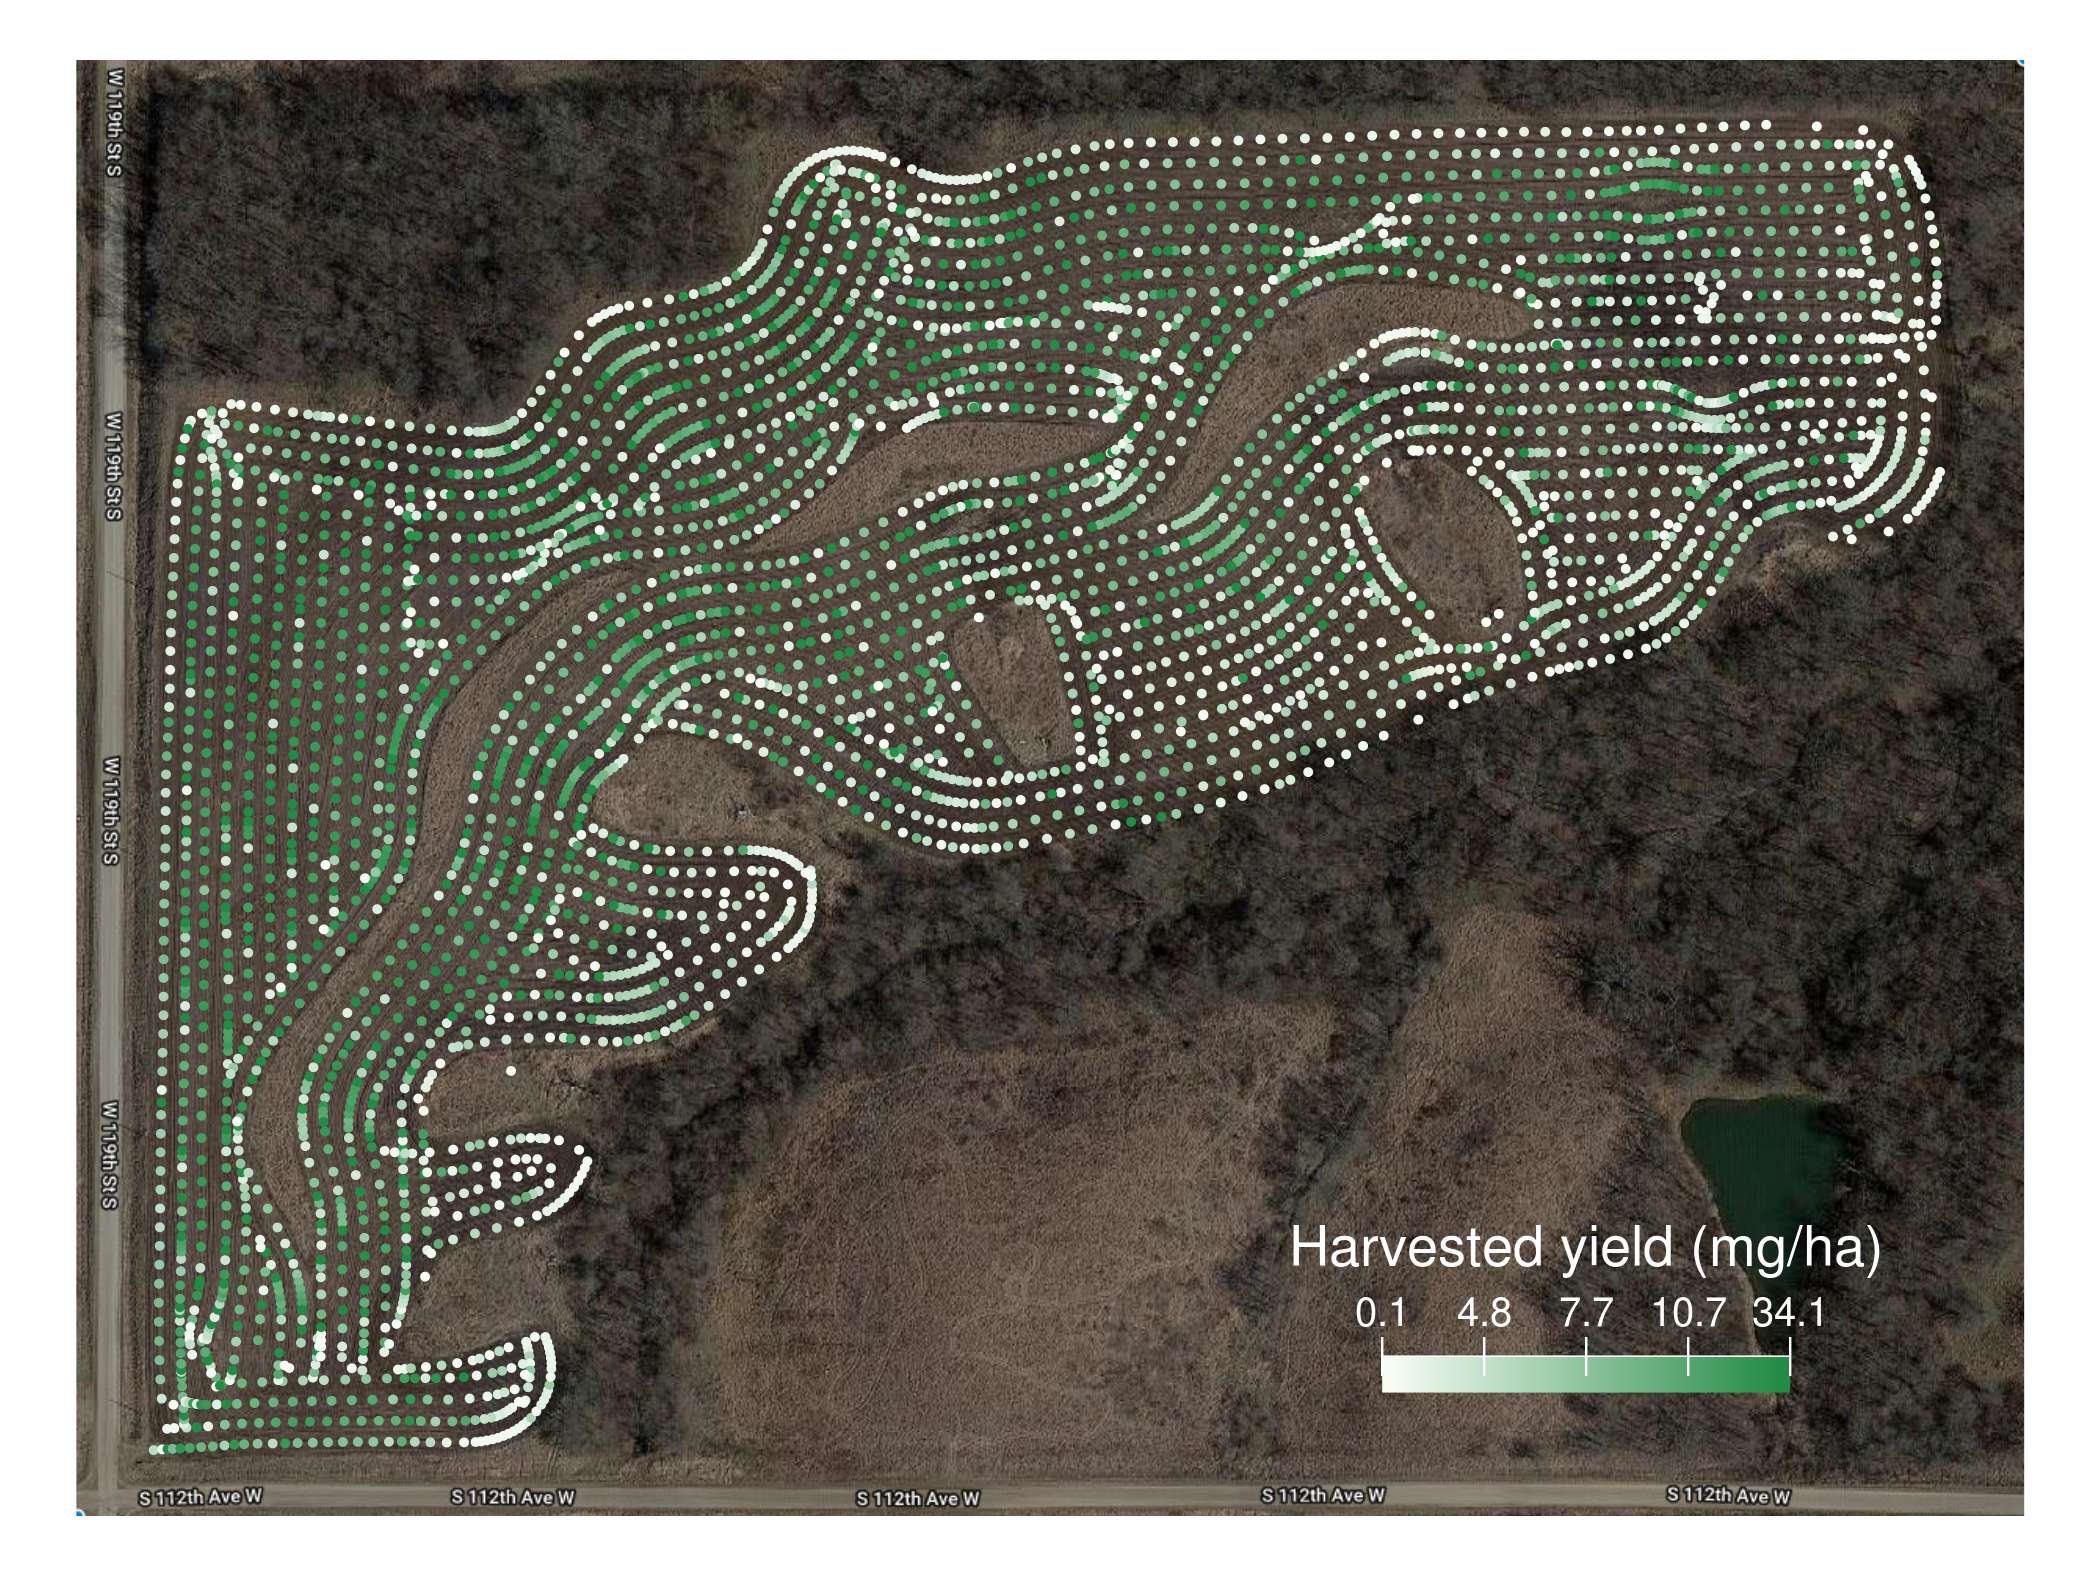
\includegraphics[width=0.75\textwidth]{appendix/basswood_2012_res5_1_points_vehicle}
%         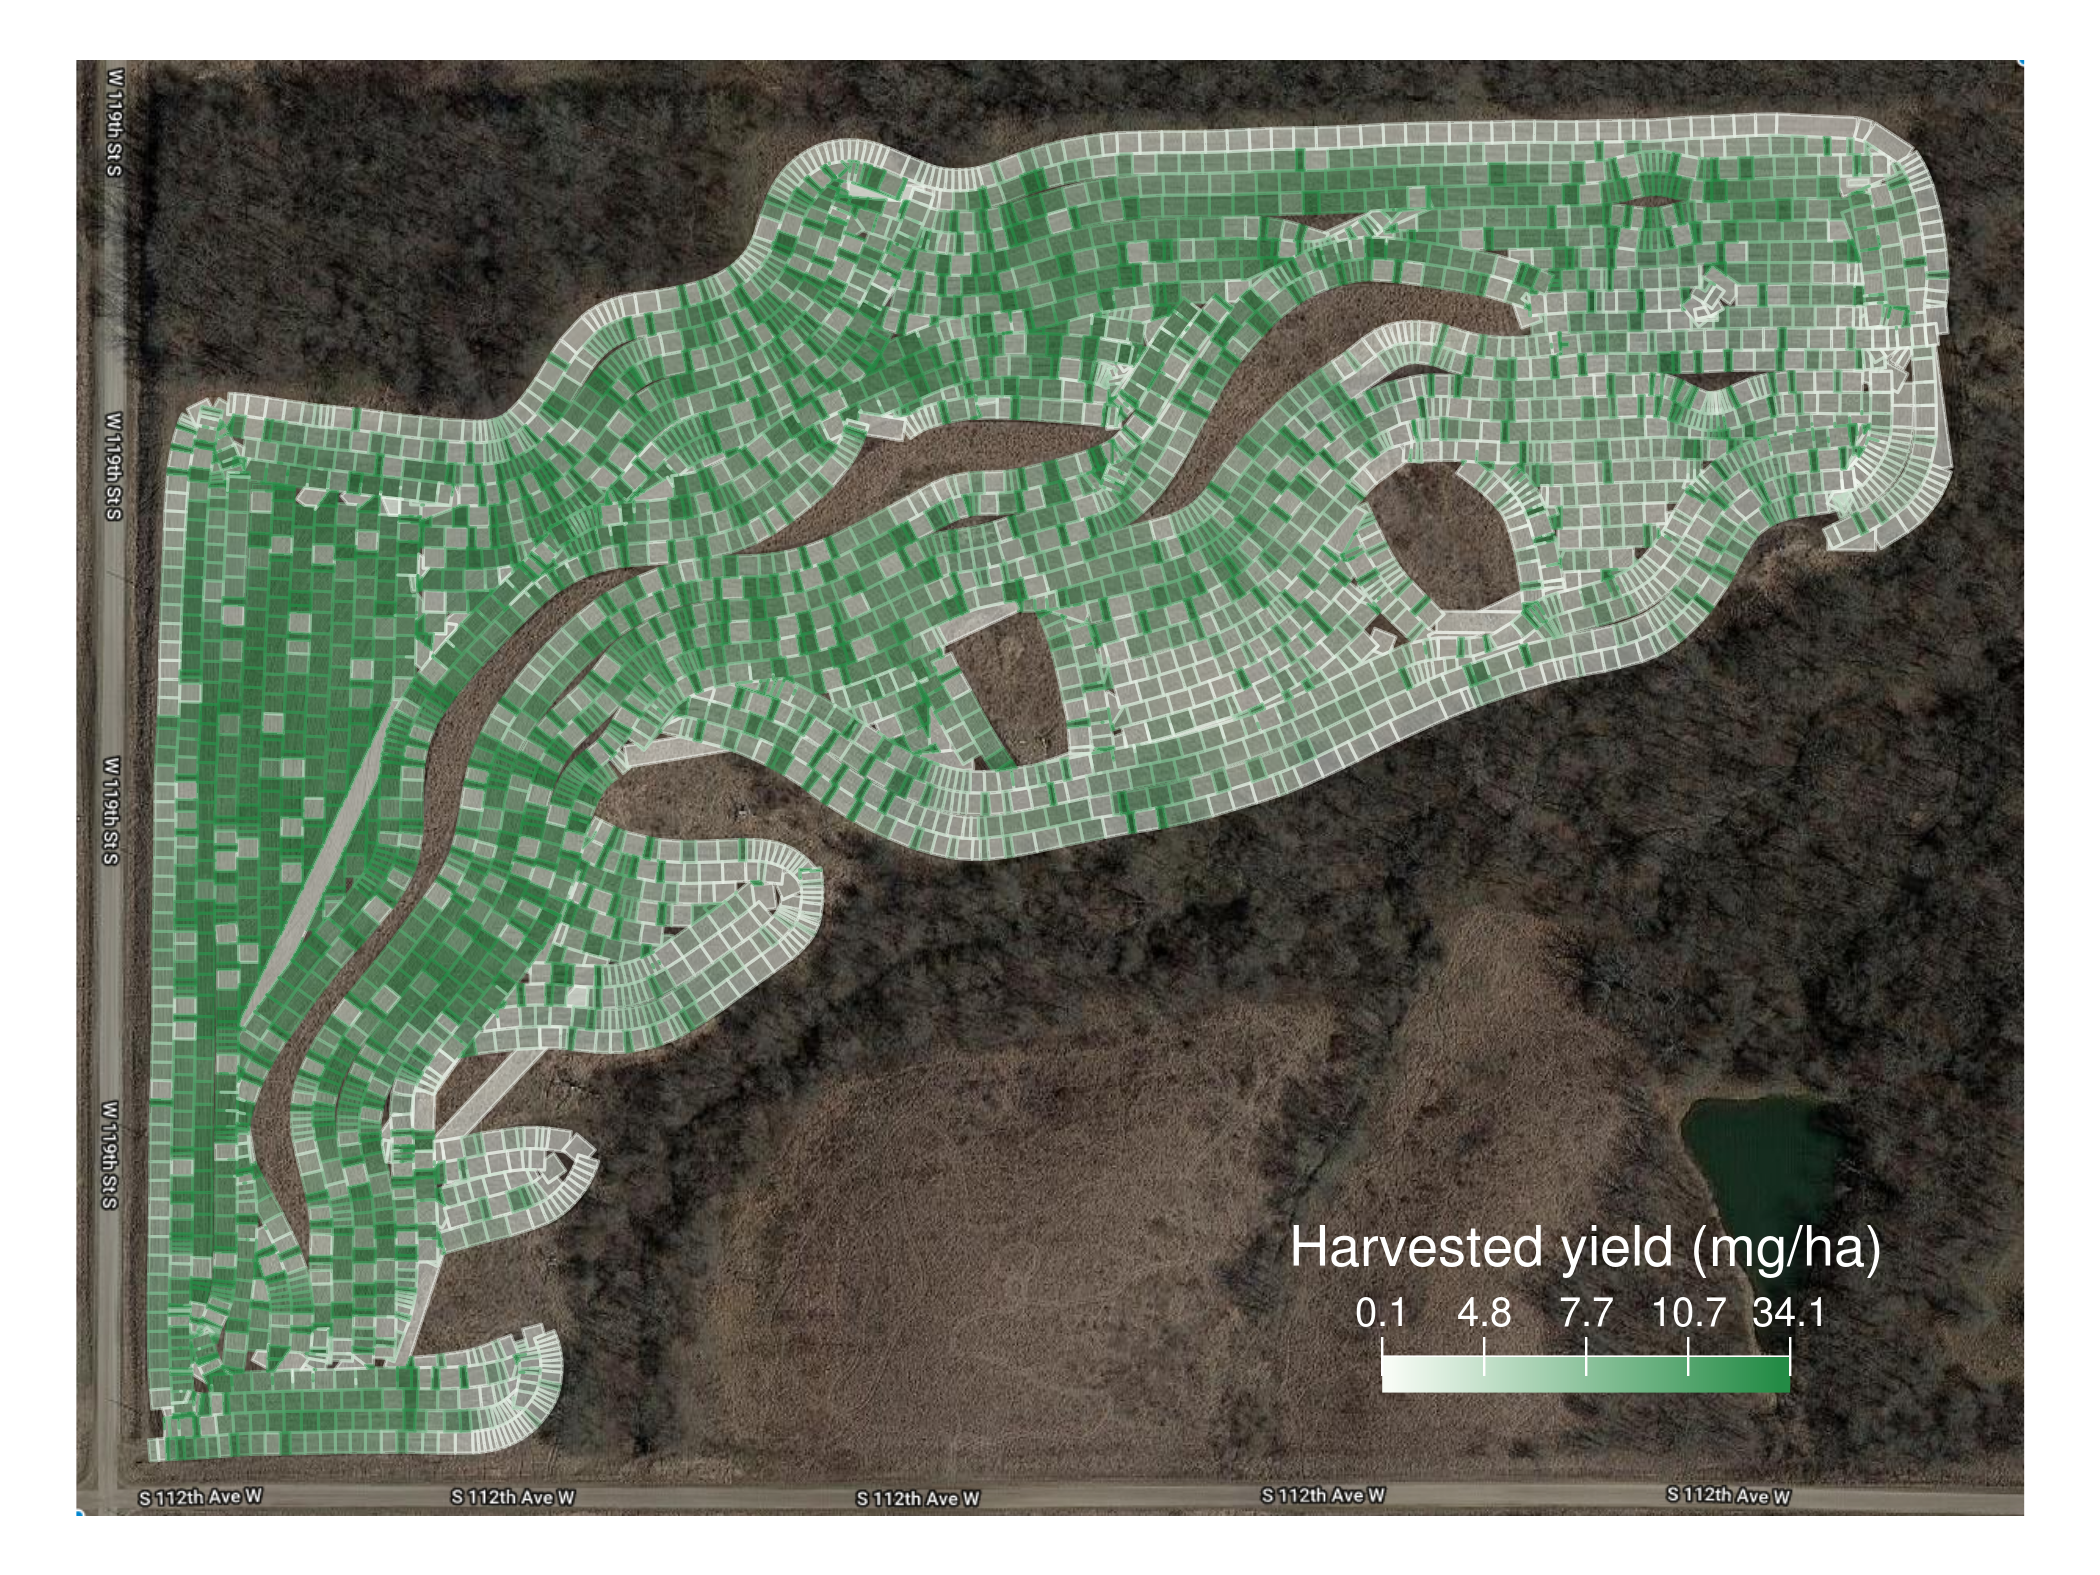
\includegraphics[width=0.75\textwidth]{appendix/basswood_2012_res5_1_reshaped}
%         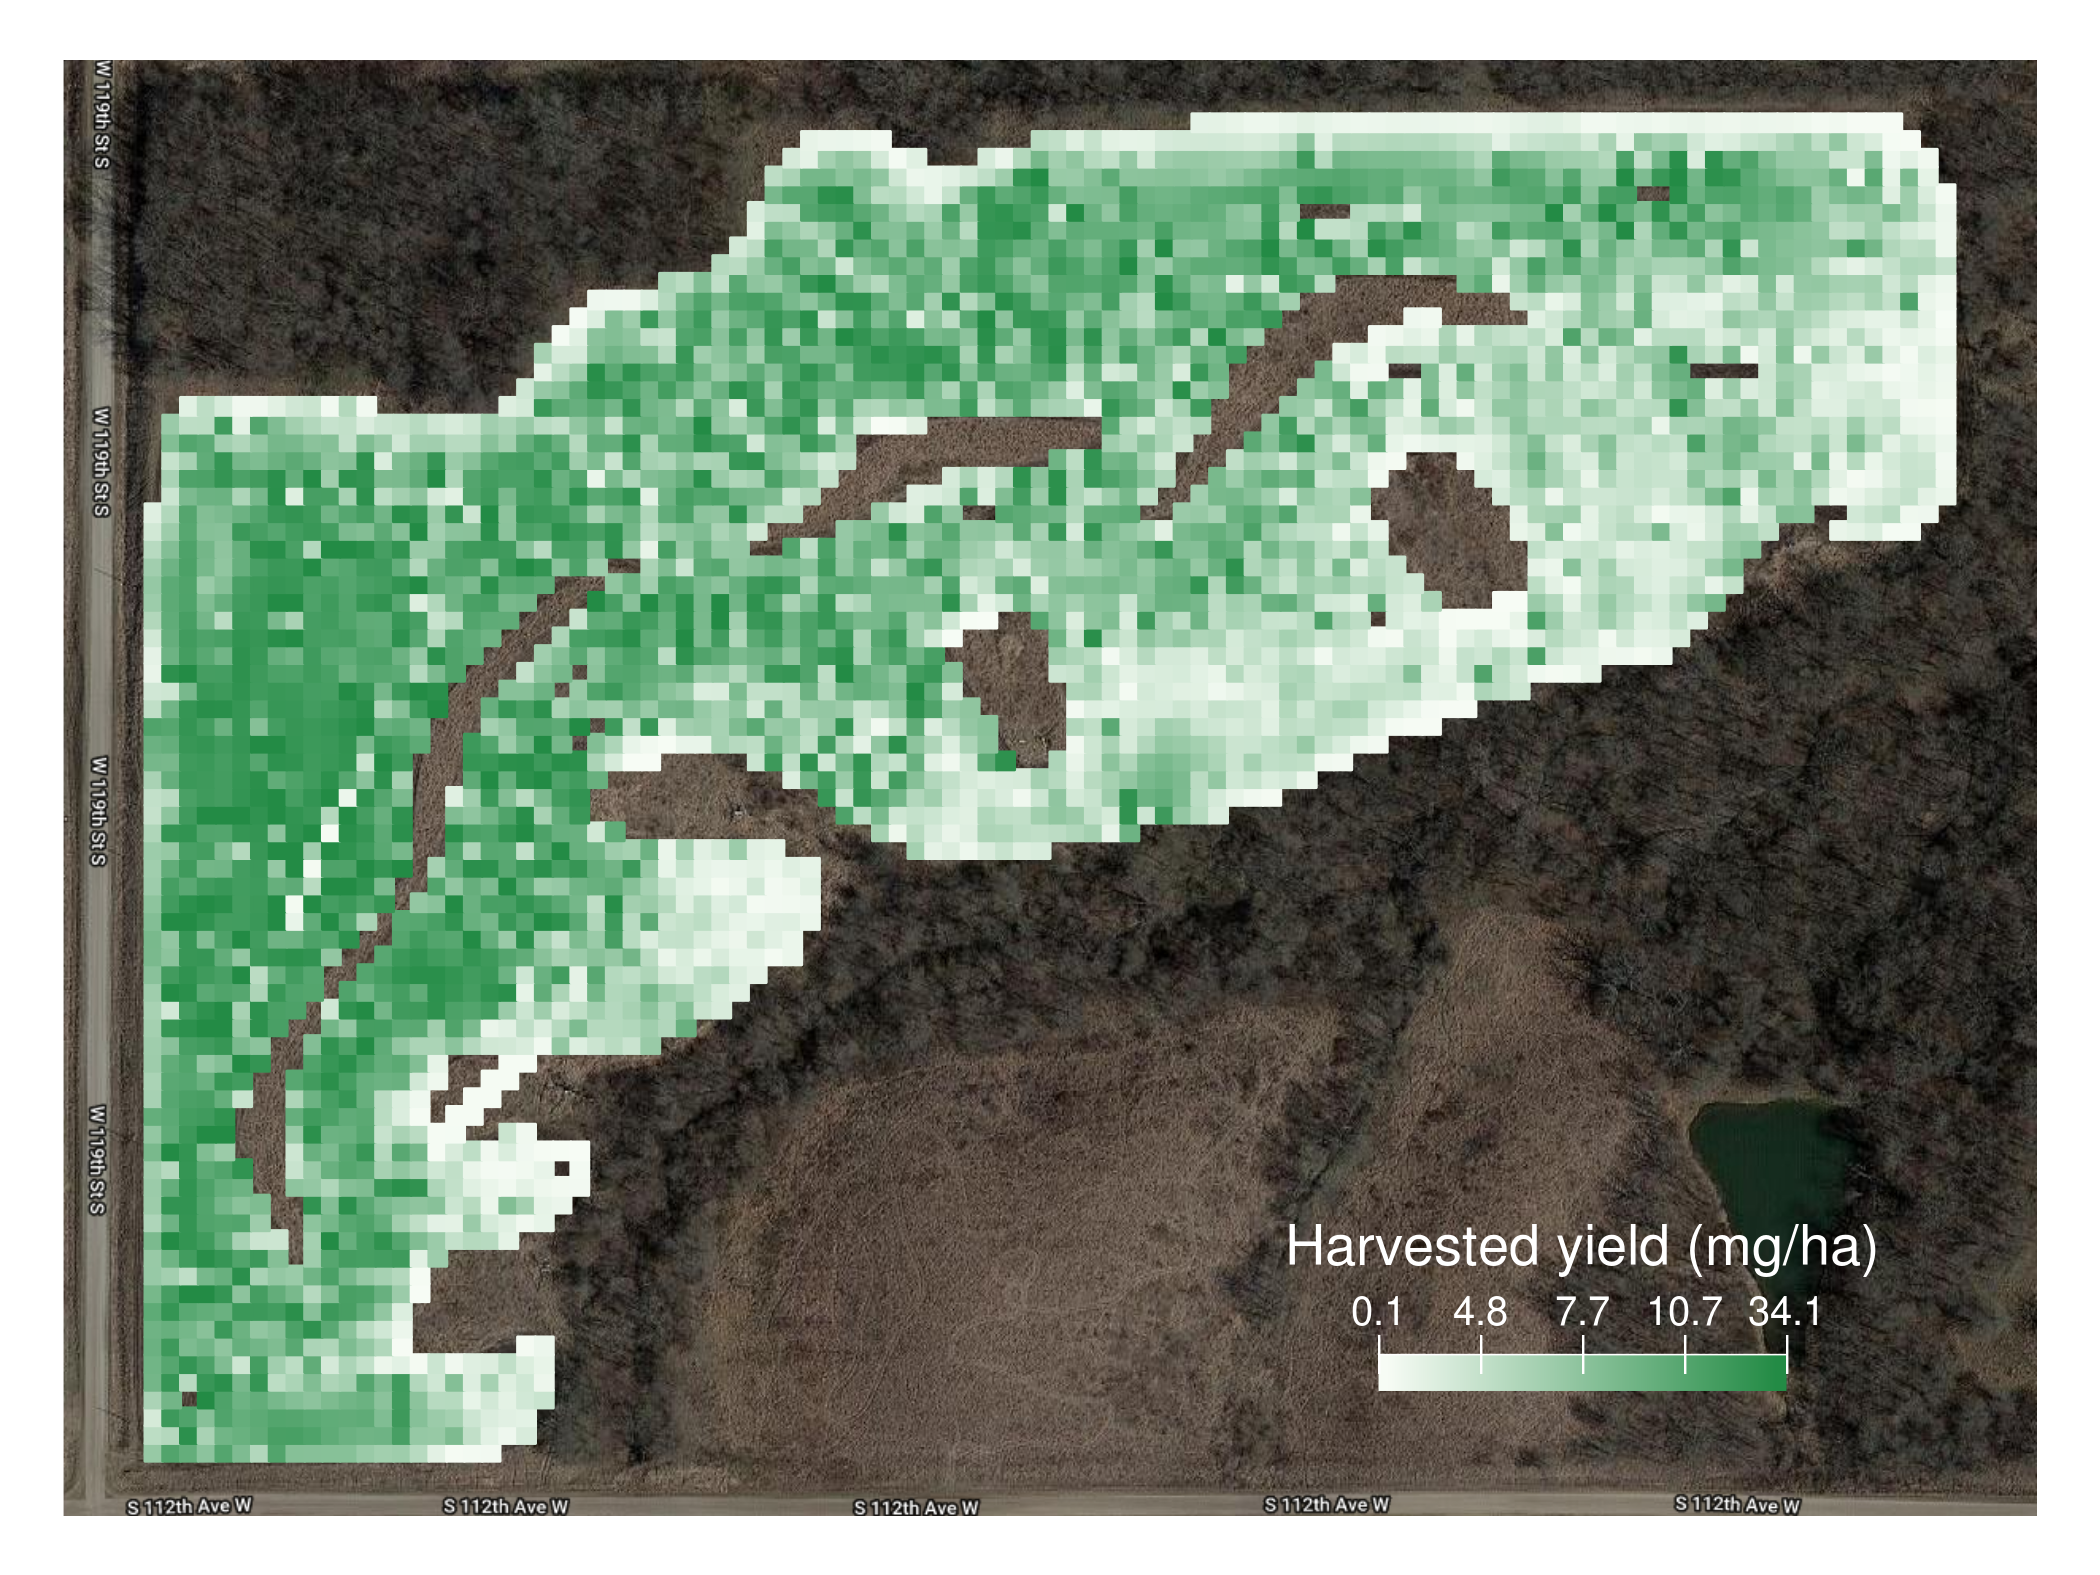
\includegraphics[width=0.75\textwidth]{appendix/basswood_2012_res5_1_aggregated}
%     \end{minipage}\hfill
%     \begin{minipage}{0.49\textwidth}
%         \centering
%         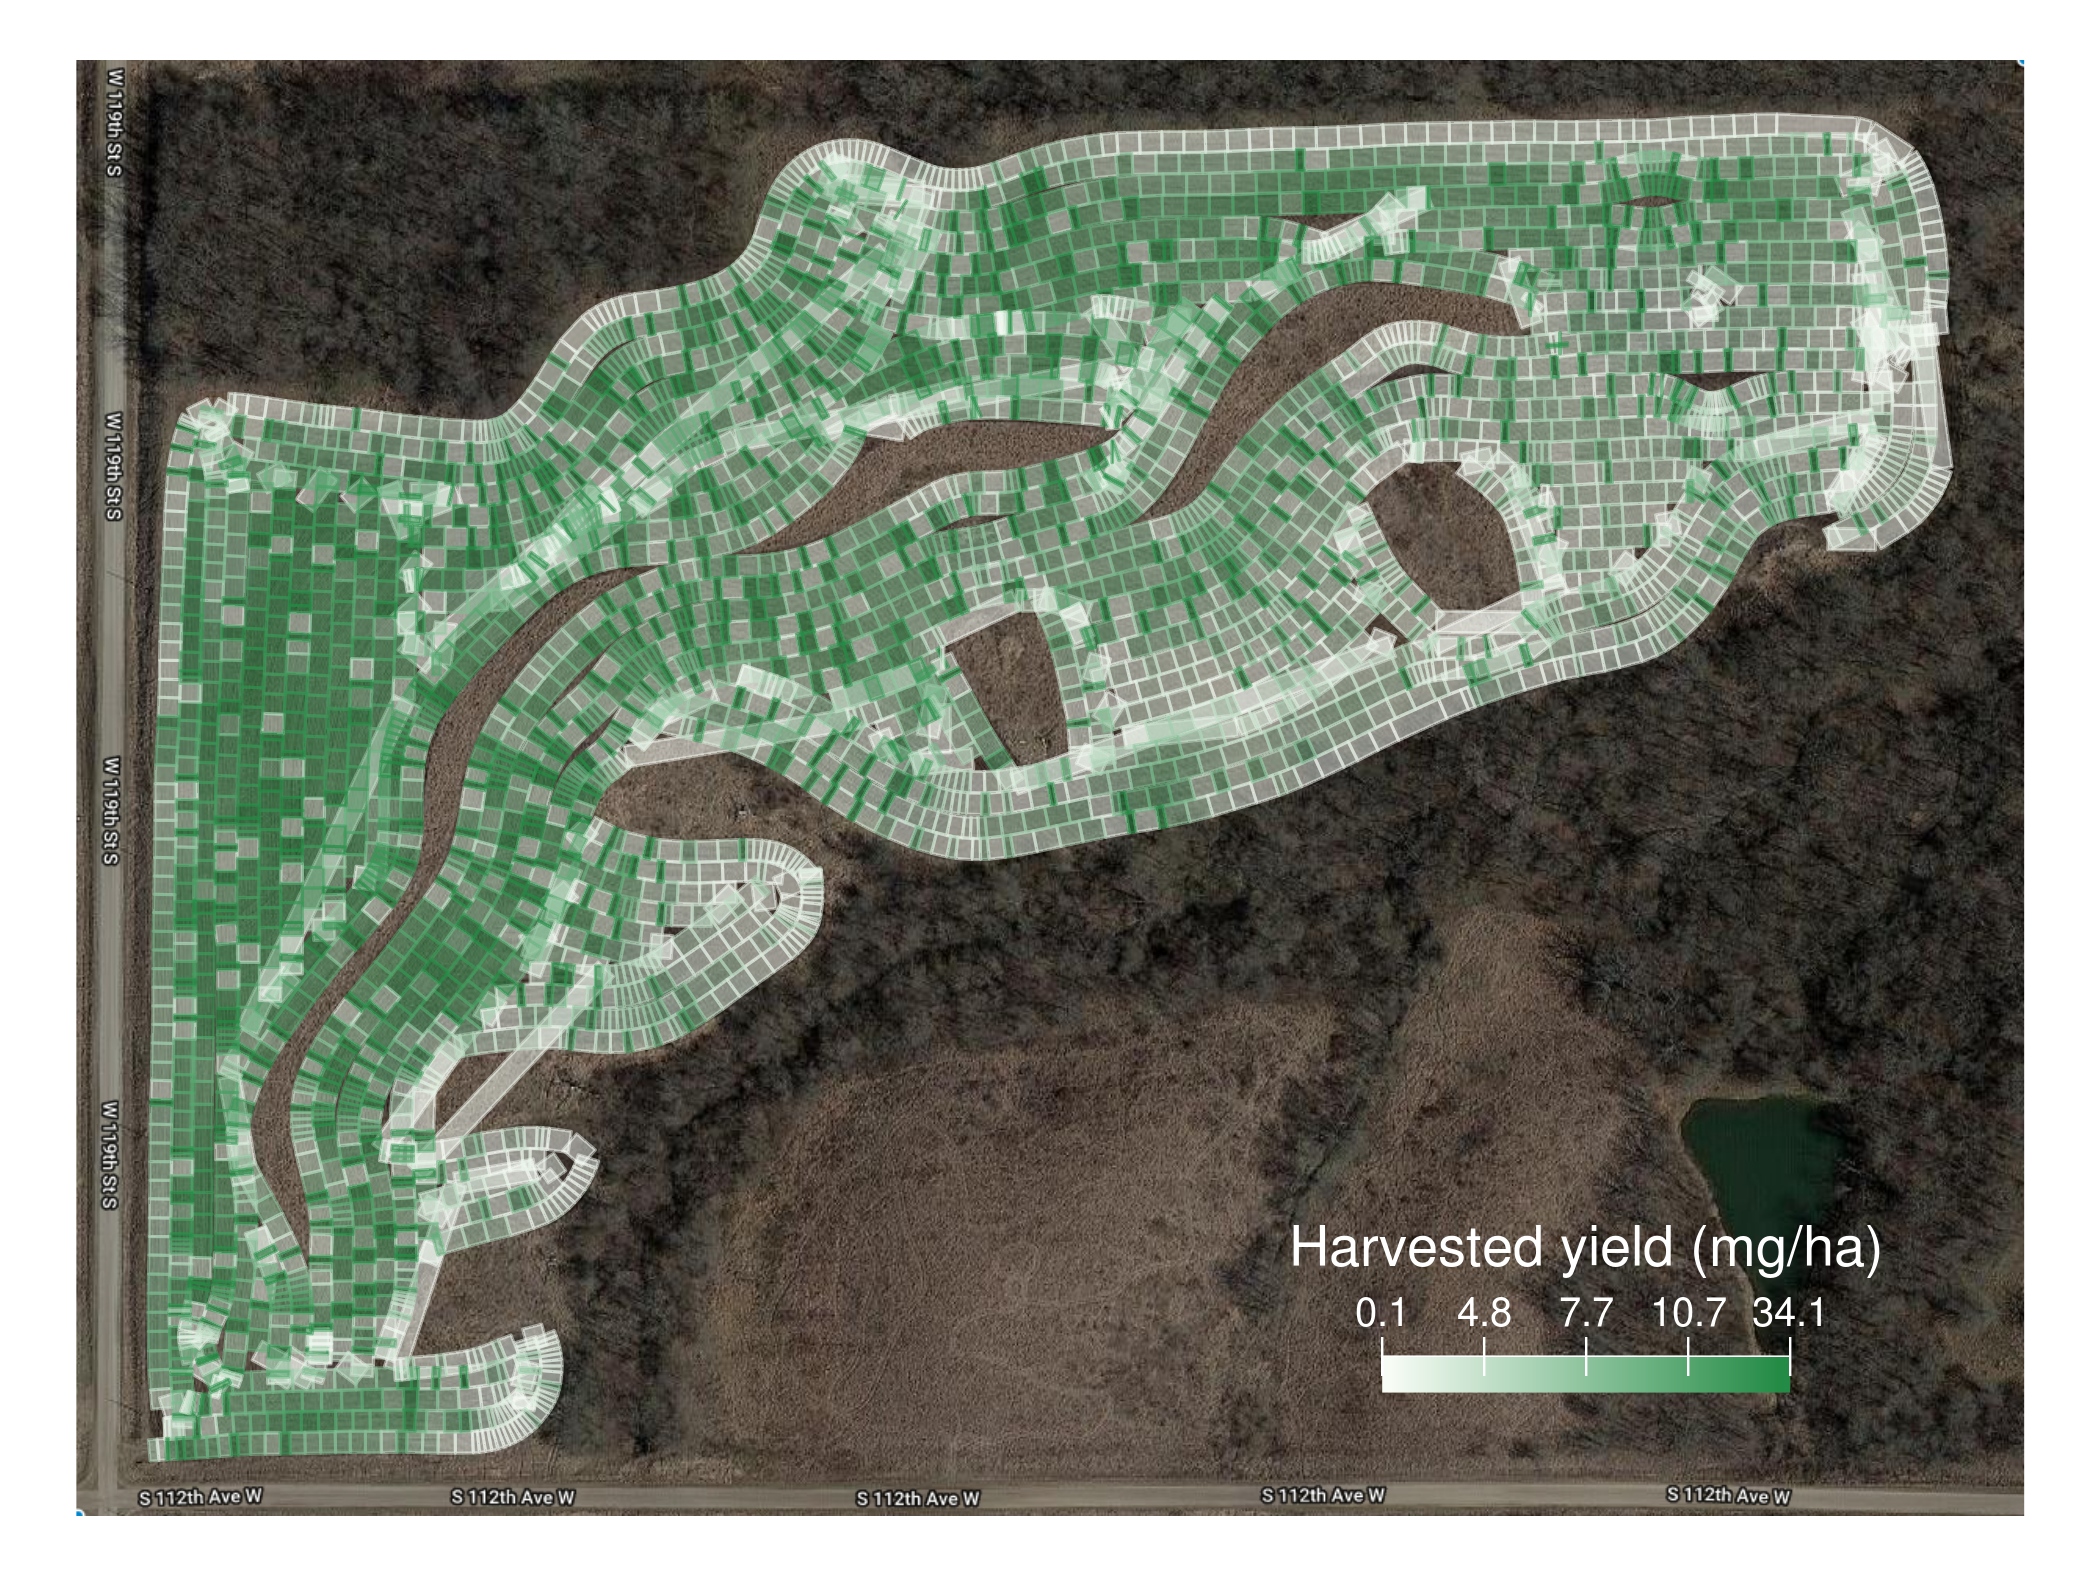
\includegraphics[width=0.75\textwidth]{appendix/basswood_2012_res5_1_polygons_vehicle}
%         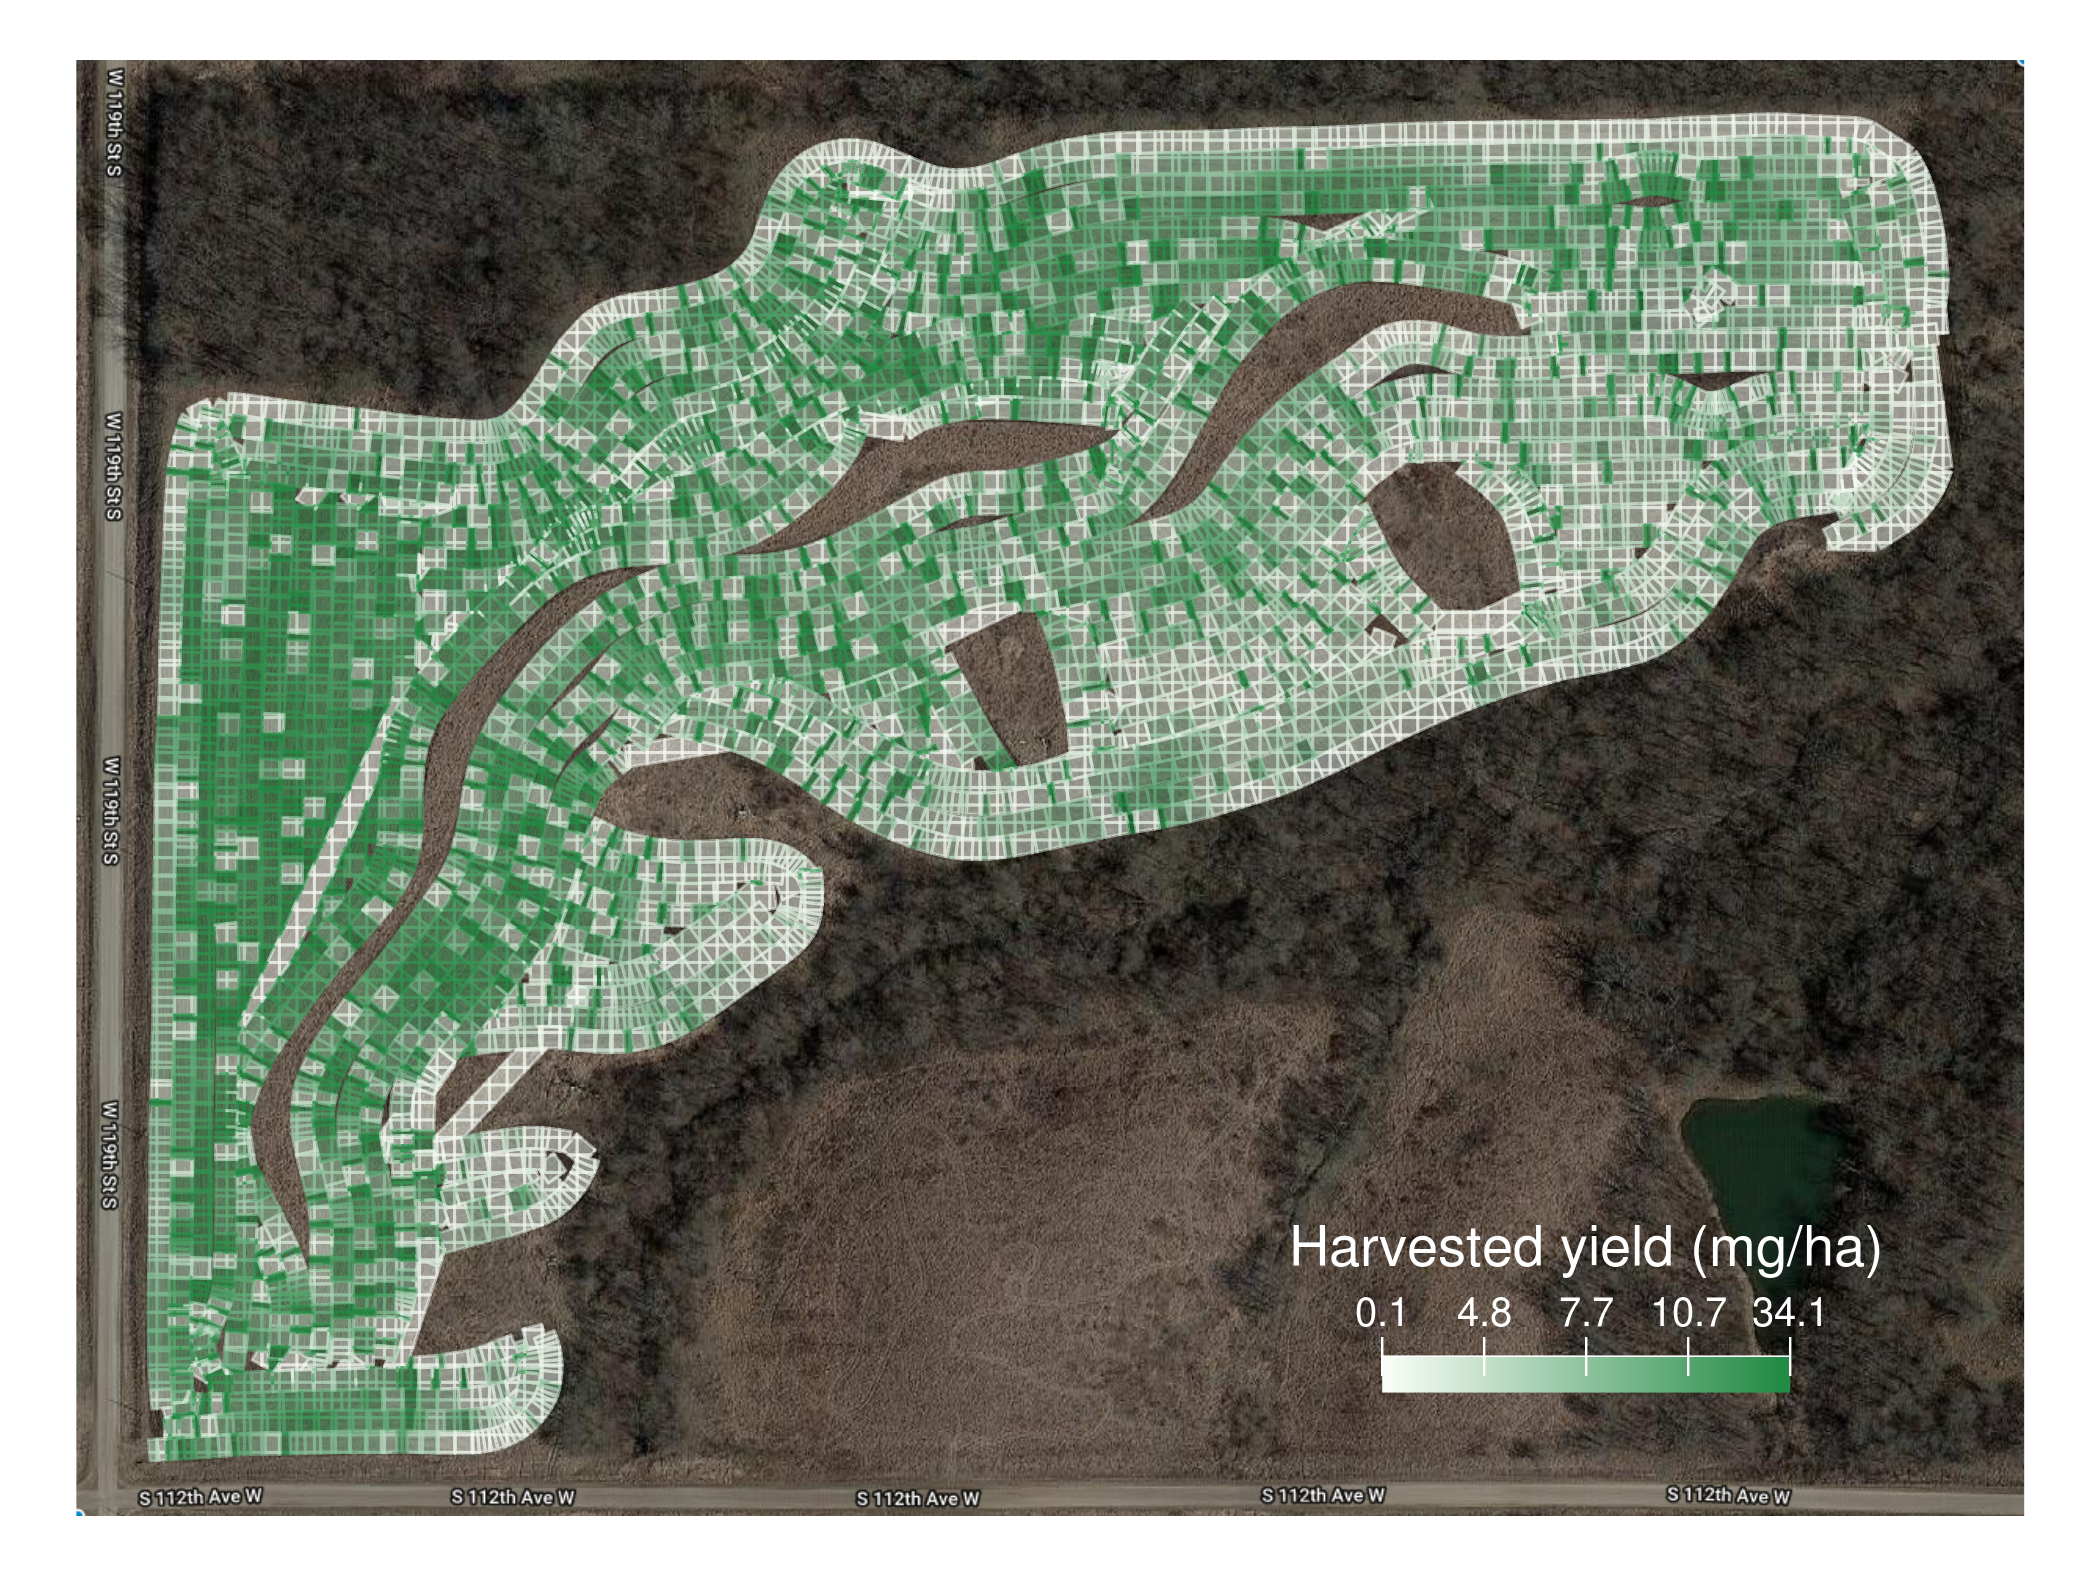
\includegraphics[width=0.75\textwidth]{appendix/basswood_2012_res5_1_chopped}
%         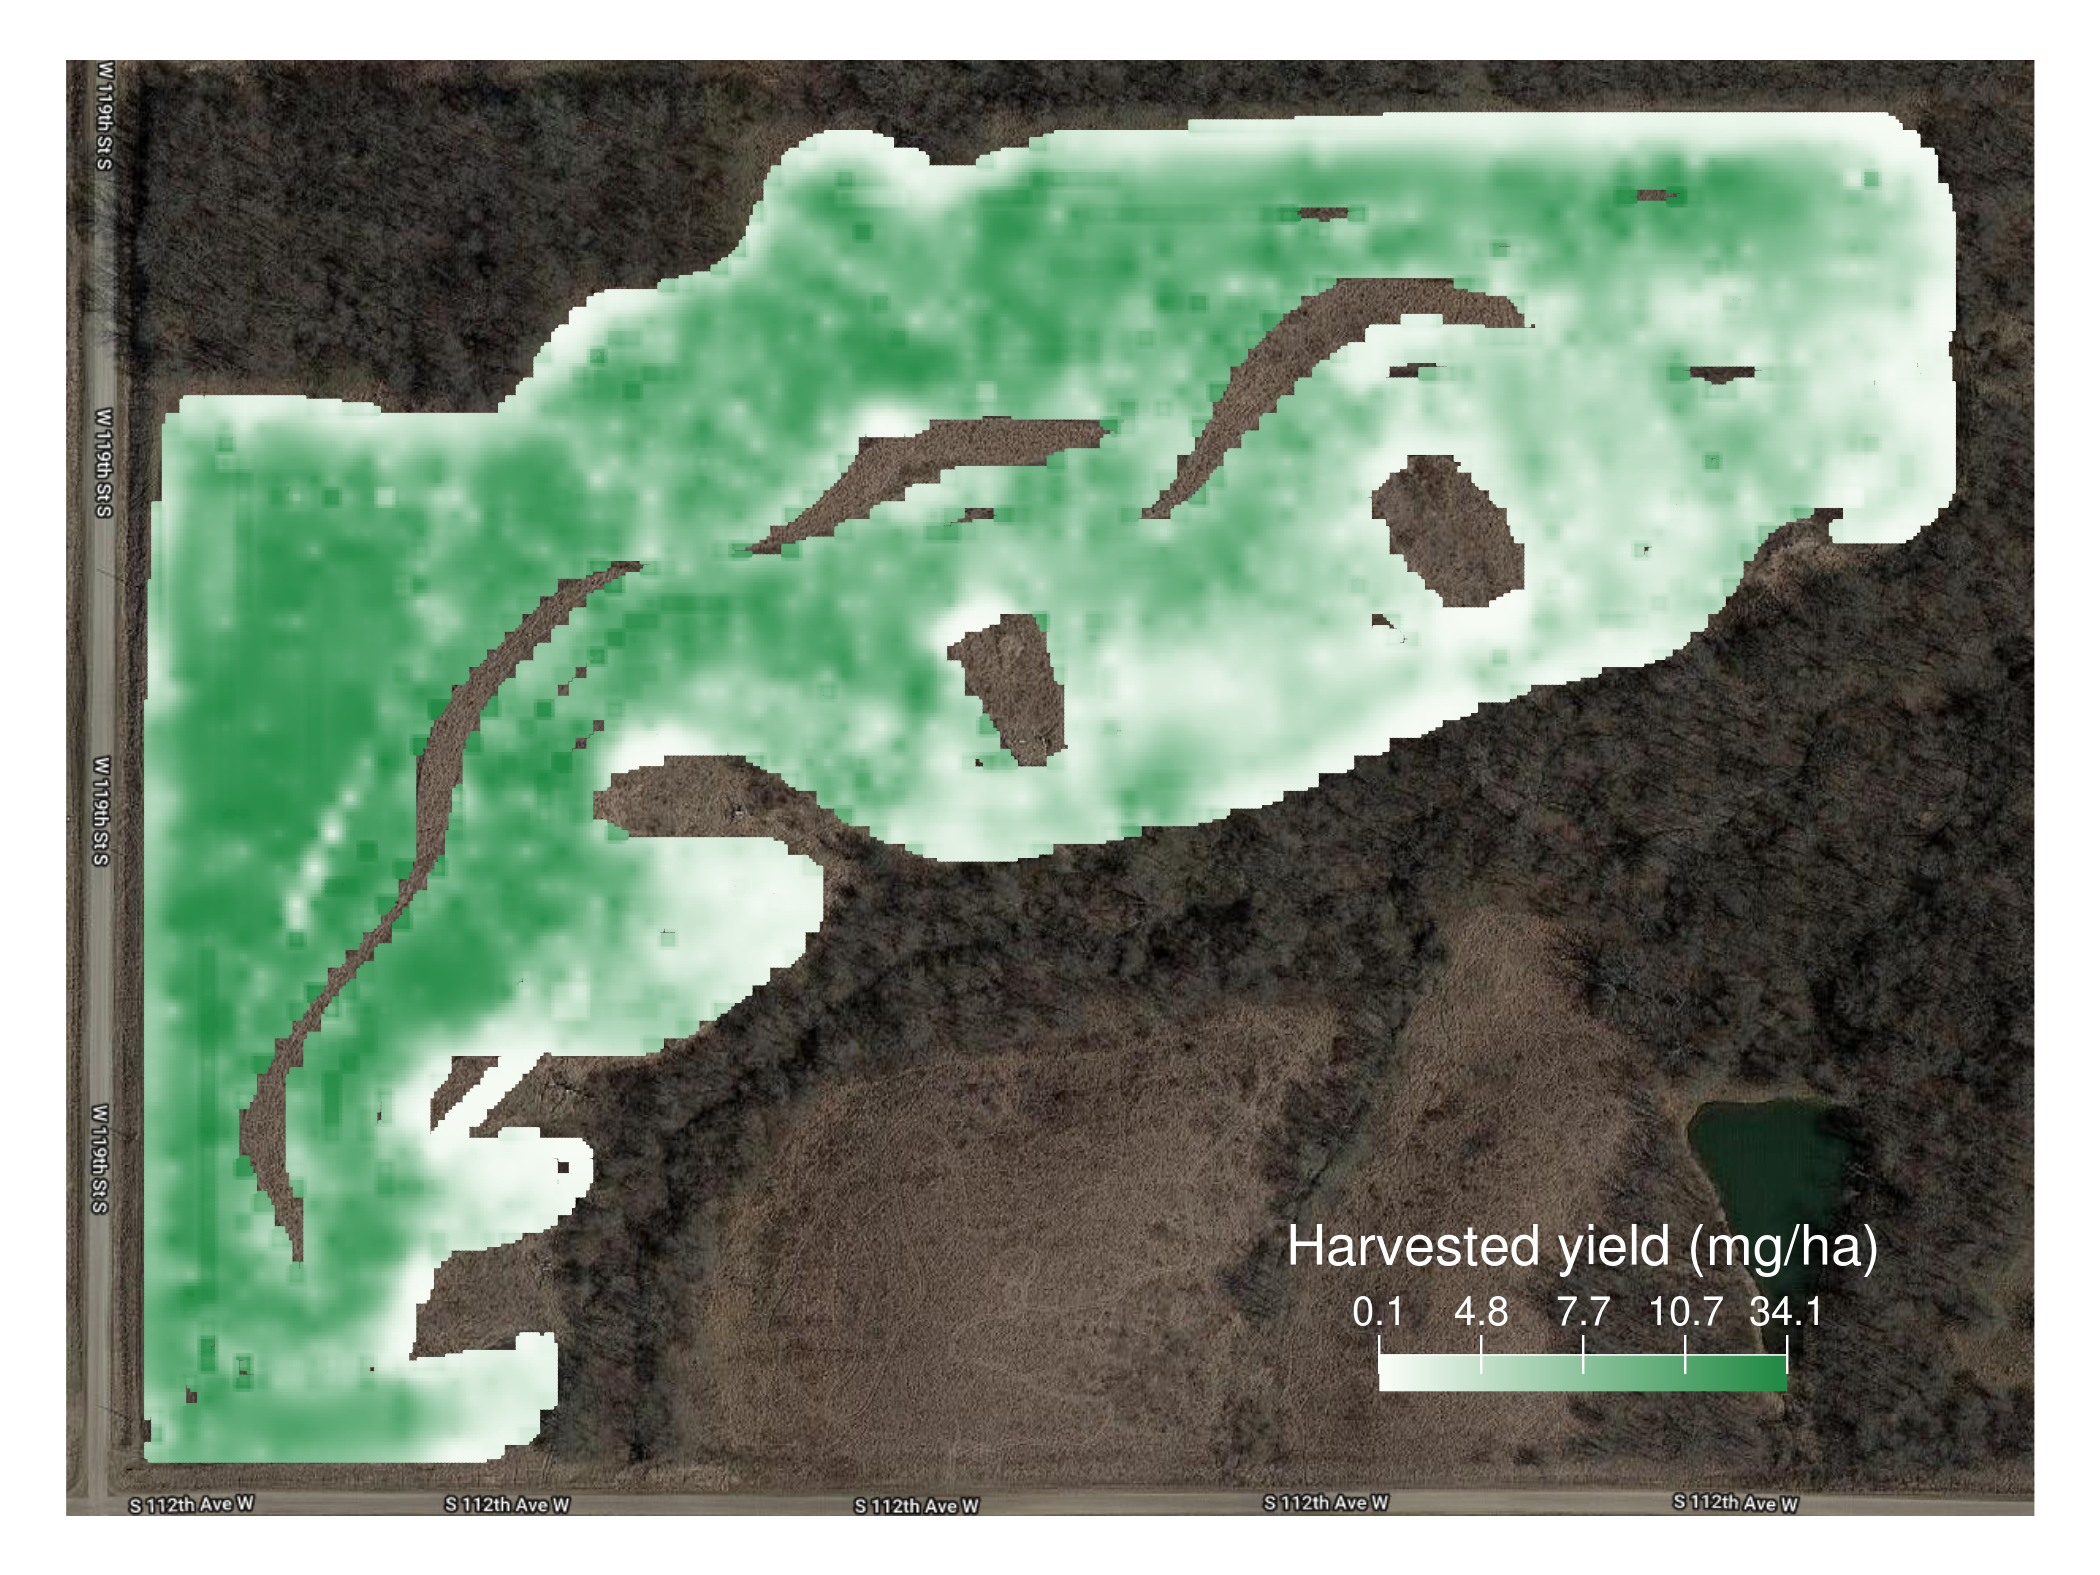
\includegraphics[width=0.75\textwidth]{appendix/basswood_2012_res5_1_smoothed}
%     \end{minipage}
%     \caption[Step-by-step visualization of the algorithm for one field]{Every step progression. Point and intersection maps
%       in the top row, reshaped and clipped maps in the middle row, and
%     aggregated and smooth maps in the bottom row.}
%     \label{fig:basswood2012-all-steps}
% \end{figure}

%%% Local Variables:
%%% mode: latex
%%% TeX-master: "../thesis"
%%% End:
